\documentclass[11pt]{article}
\usepackage{geometry}                
\geometry{letterpaper}                   

\usepackage{graphicx}
\usepackage{amssymb}
\usepackage{epstopdf}
\usepackage{natbib}
\usepackage{amssymb, amsmath}
\DeclareGraphicsRule{.tif}{png}{.png}{`convert #1 `dirname #1`/`basename #1 .tif`.png}

%\title{Title}
%\author{Name 1, Name 2}
%\date{date} 

\begin{document}



\thispagestyle{empty}

\begin{center}
\includegraphics[width=5cm]{ETHlogo.eps}

\bigskip


\bigskip


\bigskip


\LARGE{ 	Lecture with Computer Exercises:\\ }
\LARGE{ Modelling and Simulating Social Systems with MATLAB\\}

\bigskip

\bigskip

\small{Project Report}\\

\bigskip

\bigskip

\bigskip

\bigskip


\begin{tabular}{|c|}
\hline
\\
\textbf{\LARGE{Learning in Simulated Agent-based Financial Markets}}\\
\\
\hline
\end{tabular}
\bigskip

\bigskip

\bigskip

\LARGE{Daniel Keyes \& Christophe Piveteau \& Isabella Susnjara}


\bigskip

\bigskip

\bigskip

\bigskip

\bigskip

\bigskip

\bigskip

\bigskip

Zurich\\
December 2016\\

\end{center}



\newpage

%%%%%%%%%%%%%%%%%%%%%%%%%%%%%%%%%%%%%%%%%%%%%%%%%

\newpage
\section*{Agreement for free-download}
\bigskip


\bigskip


\large We hereby agree to make our source code for this project freely available for download from the web pages of the SOMS chair. Furthermore, we assure that all source code is written by ourselves and is not violating any copyright restrictions.

\begin{center}

\bigskip


\bigskip


\begin{tabular}{@{}p{1.3cm}@{}p{5cm}@{}@{}p{5cm}@{}@{}p{5cm}@{}}
\begin{minipage}{3cm}

\end{minipage}
&
\begin{minipage}{6cm}
\vspace{2mm} \large Daniel Keyes

 \vspace{\baselineskip}

\end{minipage}
&
\begin{minipage}{6cm}

\large Christophe Piveteau

\end{minipage}
&
\begin{minipage}{6cm}

\large Isabella Susnjara

\end{minipage}
\end{tabular}


\end{center}
\newpage

%%%%%%%%%%%%%%%%%%%%%%%%%%%%%%%%%%%%%%%



% IMPORTANT
% you MUST include the ETH declaration of originality here; it is available for download on the course website or at http://www.ethz.ch/faculty/exams/plagiarism/index_EN; it can be printed as pdf and should be filled out in handwriting


%%%%%%%%%% Table of content %%%%%%%%%%%%%%%%%

\tableofcontents

\newpage

%%%%%%%%%%%%%%%%%%%%%%%%%%%%%%%%%%%%%%%



\abstract{
We present an agent-based model designed to simulate trading dynamics of a financial market. The behaviour of the individual agents is determined by three parameters, which we dub ``conservativeness'', ``influencability'' and ``noisiness''. This parameter space allows one to produce agent behaviour that can mimic a continuous range of strategies encompassing momentum traders and noise traders. We perform repeated simulation rounds; in each simulation, agents place bids, and price formation is performed by determining a market clearing price and executing admissible bids. Finally we analyze multiple learning strategies so that agents optimize their success (expected net worth) in the simulation. We use a heuristic method for performing Gradient Descent optimization. As this optimization suffers from the curse of dimensionality, we reduce the agent paramater space to one dimension for computational reasons. In one dimension the strategy distribution converges stably to a characteristic Gaussian-like distribution, independent of the initial agent strategy distribution.
}
\newline

\section{Individual Contributions}

\section{Introduction and Motivations}
\subsection{Financial Actor Behaviour}

Due to the hyper-competitive nature of financial markets and their near-instantaneous price adjustments, prominent academics assumed that individual rationality in decision making leads to efficient price outcomes \citep{zeckhauser1991nonrational}. This theory is known as the Efficient Market Hypothesis (EMH), which assumes all market information is incorporated at the price, hence assets trade at their intrinsic value and `beating the market' becomes impossible. \\
Under such conditions, since all agents are perfectly informed, picking undervalued stocks via fundamental (relating to macroeconomic factors) or technical (depending on price movement and volume of past trading activity) market analysis is redundant. However, although consensus about the efficiency of markets has yet to be reached, there is some disbelief of the ‘rationality of the markets’ especially after the 2007-09 crisis. This perspective suggests that external market factors, such as trading strategies and the resulting asset prices, are the underlying behavioural parameters. This warrents the investigation of varied agents and their effect on the market. \\

\subsection{The Case for Simulation}
The importance of understanding the dynamics in a financial market and the parameters that determine investor behaviour is manifested in the various policy efforts that seek to maintain integrity in the financial system.\\
For instance, in order to secure market confidence, regulate foreign participation and prevent collusion, policy makers have become increasingly interested in identifying dominant trading strategies and the social effects that level the playing field. The market composition plays a significant role in the predictive analysis as it is likely to exacerbate inherent financial dynamics. Examples are the speculative bubbles experienced in 2000 and 2007 as observed by \citet{kaizoji2015super}. \\
One of the earliest works similar to this project is \citet{de1990noise}, which uses an agent-based economic model. Further related works that use the same model have mostly investigated emerging market characteristics (formation of demand/supply or characteristic price formation). Since the agent-based model has proven its usefulness in modelling market characteristics we feel comfortable to adopt and expand the proposed model in order to study how emergent market characteristics propagate back to the agent as in how they adapt their strategies.

\section{Description of the Model}

\subsection{Market Conditions and Trading Mechanism}
We use an agent-based model closely based on \citet{raberto2001agent} to simulate a financial market with a market-clearing price formation mechanism. Our main objective is to understand the evolution of market dynamics as agent strategies change due to social learning among agents. \\
At the start of the simulation, wealth and assets are uniformly distributed among agents, who have heterogenous strategies. We adopted the assumption that the market comprising these agents is endowed with a finite amount of wealth and assets, which enacts realistic constraints on agents' decision-making. \\
The base structure of our model is an artificial financial market where agents trade an asset in each of $T$ trading periods per simulation. At every trading interval, agents choose to either buy or sell, and they simultaneously place limit orders at individual limit prices. Limit prices are prices specified by the agents at which assets are marketed, but where transactions may not be executed if the market price set by investors is not met during the trading period. This induces a demand and supply curve. The market clearing price is computed at the intersection of demand and supply, and admissible transactions are cleared as described in further detail in the following paragraphs. \\
The amount of total traded assets per time step is computed by aggregating individual orders. Each agent considers how many assets she wants to own in the following time step. This value is drawn from a normal distribution with mean $\mu_S$ and standard deviation $\sigma_S$:

\begin{equation}
\mu_S = \text{currentAmountOfAssets} * (1 + (\text{marketPrice} - \text{meanMarketPriceOverNTimesteps}) * \text{agentConservativeness} + \text{priceMomentum} * \text{agentInfluencability}, \sigma_S = \text{agentNoisiness})
\end{equation}
We see that $\mu_S$ starts out to be around the current amount of assets of the agent. There are two forces influencing $\mu_A$: If the market price is higher(lower) than the average in recent history, then the agent is more likely to sell(buy). If a lot of people are buying(selling) and thus the market price momentum is high(low) the agent is more likely to buy(sell). These two forces are weighted by two agent parameters: its conservativeness and its influencability. A third parameter governs the behaviour of our agents, namely  noisiness.\\
Finally the order price is also taken from a normal distribution with mean $\mu_P$ and standard deviation $\sigma_P$:

\begin{equation}
\mu_P = 0.99 * \text{currentAssetPrice} \text{if the agent is buying}
\end{equation}
\begin{equation}
\mu_P = 1.01 * \text{currentAssetPrice} \text{if the agent is selling}
\end{equation}
\begin{equation}
\sigma_P = \text{const} * \text{marketVolatility}
\end{equation}

After agents place their bids, the model undergoes price formation. As with [1], we would like to find a market clearing price price p* for which the highest number of bids can be satisfied. Specifically, we would like the total amount of sell bids below the price to be equal to the total amount of buy bids above the price. Given a sorted list of buy and sell orders, this can be performed in linear time by using a two-pointer implementation. We iterate from the lowest-priced sell order and from the highest-priced buy order, matching pairs of orders as we go, until the current buy price is less than the current sell price. In the case that more satisfiable buy orders exist than sell orders (or vice-versa), the successful bids are chosen randomly. All orders are then executed at p*, the average of the highest matched sell order and lowest matched buy. Then the next timestep starts and the process repeats. \\
We conducted three experiments, one for each learning strategy. For each experiment we ran multiple simulations, where each initiation starts with the same initial conditions, i.e. type of traders, asset and wealth distribution.  The beginning of each period initialises the agents’ endowments of money and assets, which are normally distributed, and the state of nature. Information about the states of nature is publicly available to all agents, such as…?Borrowing and short selling is prohibited and agents cannot exceed their budget constraint at any point in time. Furthermore, there is no mechanism for money creation.\\

\subsection{Agents}
The design of our agents closely follows XYZ’s (author) traders, which uses XX heuristic to give us an understanding of how agent parameters change and interact in market phenomena. Simple heuristics allow us to examine the interactions among and within agent parameters and how trading strategies change over time. \\
In our model all agents are risk neutral and seek to maximise their end-of-trading-period wealth and the expected value of their portfolio. For this end they choose between cash and wealth and only buy assets when the clearing price is low in relation to their mean (vice verca sell when the price is high in relation to their mean.) \\
We do not model utility functions, but preferences for assets occur due to differences in the influencability of market factors and conservatieness… \\
Agents submit orders in the same manner, outlined above , but differ in the way they determine the expected value of the asset, which we call the ‘base price’ (the fundamental cost of the asset to the trader).  \\
There is a continuous set of types of agents with a normal distribution of agent parameters, which also determines how they form their forecast. Traders can vary along the spectrum of influencability and conservativeness, which means… This agent design is inspired by the differences in fundamentalist and technical traders, which trade according to…., respectively. F use… they form their base price by… and aim to buy or sell if the base price is higher or lower than the market determined asset price, which signifies an under- or overvalued stock from their point of view. These traders continuously monitor market activities, update their parameters and adust their trading position accordingly. Their trading activities come to an end when they outspend their budget constraint or … \\
Technical traders use the current time periods and past return values as a proxy measure for future returns. (e.g. if at time t the two most recent transaction prices are pt and pt1, then a momentum trader's forecast of the next transaction price is simply pt (pt=pt1).  \\
- wealth is reseat after every learning step to initial wealth distribution. Because if you don't do this then agents that are bad at the bedinning are bad forever and have no change to improve. 
Learning	
MLS
Gradient
Naive
- Agents undergo ten learning steps in our model. 

Agents also undergo a learning process. The model is run for a specific number of time steps, then a ranking of the agents is done considering their final owned wealth. Depending on how successful each agent was in that ranking, she will adapt her parameters: A successful agent will only slightly change its parameters, while less successful agents will vary them more strongly.

In order to create the optimization algorithms of our agents we approximate a continuously differentiable function using the Moving Least Squares (MLS) method. For this we approximate a continuous function from the scattered point sample of our agents’ influencability/wealth distribution by calculating weighted least squares (WLS) measures from an arbitrary point in the parameter space. We use a Gaussian weighting evaluated at neighbouring points and normalised by their sum. The selected point is consequently moved over all agent positions in the parameter domain, a local linear fit computed and individually evaluated for each point of the sample. 

FORMULA

We decided to use this method as it this method successfully interpolates emerging data 
as was originally suggested by \citet{lancaster1981surfaces}. 

MLS converges very slowly, so we use more heuristics (here it converges faster with 1D). so now that it converges faster we see how it works in 2D. But it takes too much computational power. Interesting for future research. 







Description of MLS: DANIEL

Another optimization approach is one we developed and call Heuristic Gradient. It calculates a gradient that has no mathematical meaning, but is rather a quantity that heuristically represents in which direction the agent will want to move in order to imitate more successfull agents. \\
We enumerate our agents with the index $i$ for $i=1,...,N$. Without loss of generality we assume $N$ to be the most successfull agent and $1$ to be the least successfull agent (with regard to the total wealth owned after a simulation). We denote the net wealth of an agent $i$ as $W_i$. We consider an agent parameter $X_i$ which might for example be the influencability or the conservativeness. The gradient for all parameters is computed separately and thus we only cover the optimization of one such agent parameter. \\
We define the parameter space distance between two agents as
\begin{equation}
  d(i,j):=X_i-X_j
\end{equation}
The heuristic gradient of the $i$th agent is defined as \\
\begin{equation}\label{eq:heuristicgradient}
  G_i:=\frac{1}{C_i}\cdot \frac{N-i}{N} \cdot \sum\limits_{\substack{i=1 \\ i\neq j}}^{N}{ w_{ij} \cdot (W_j - W_i) \cdot sgn(d(i,j)) \cdot \frac{W_j}{W_N} }
\end{equation}
where the weight $w_{ij}$ is defined as
\begin{equation}
  w_{ij}:=exp(-\lambda \cdot abs(d(i,j)))
\end{equation}
and
\begin{equation}
  C_i:=\sum\limits_{\substack{i=1 \\ i\neq j}}^{N}{w_{ij}}
\end{equation}
where $\lambda$ is a constant that is chosen depending on the order of magnitdue of the agent parameter considered. \\
In the formula \ref{eq:heuristicgradient} one can see that the gradient is a weighed sum over all other agents where the weight exponentially decreases with the distance of the other agent in the agent parameter space. The gradient considers the difference of networth of the two agents as well as the success of the other agent compared to the most successful agent. Finally the gradient is multiplied by the normalized rank of the agent, meaning by $1$ for the least successfull agent and by $0$ for the most successfull agent. Therefore the more successfull an agent, the smaller its gradient will be and the most successfull agent has a gradient of $0$. \\
Finally the adaptation of the agent parameter $X_i'$ for the next time step is given by
\begin{equation}
  X_i' = X_i + N(C_1\cdot G_i, C_2)
\end{equation}
where $N(\mu, \sigma)$ is a normal draw from a normal distribution with mean $\mu$ and standard deviation $\sigma$ and $C_1,C_2$ are constants chosen appropriately for the order of magnitude of the agent parameter $P$. \\
In figure \ref{fig:heuristicgradient} one can see a few examples where a simulation is run on a given distribution of agent parameters and what the resulting gradient of the agents look like.
\begin{figure}
  \centering
  \quad
  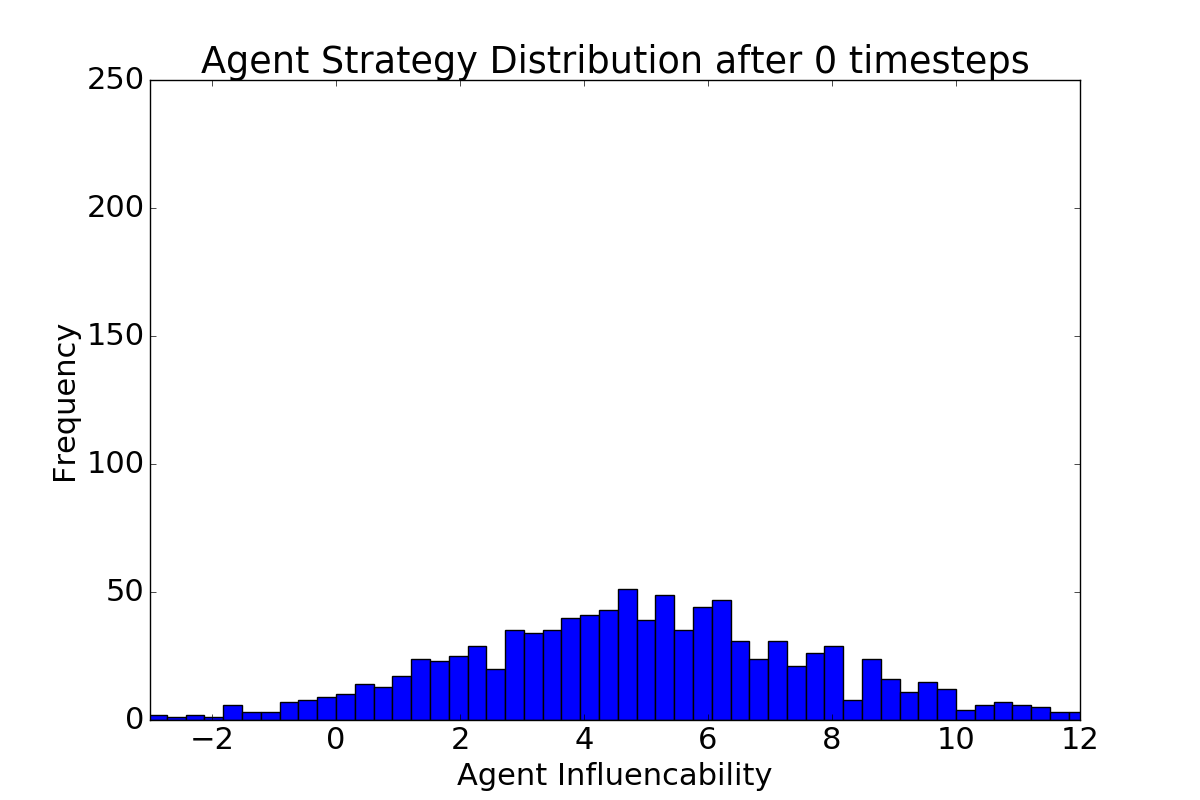
\includegraphics[width=0.45\textwidth]{figures/heuristic_gradient_example_1.png}
  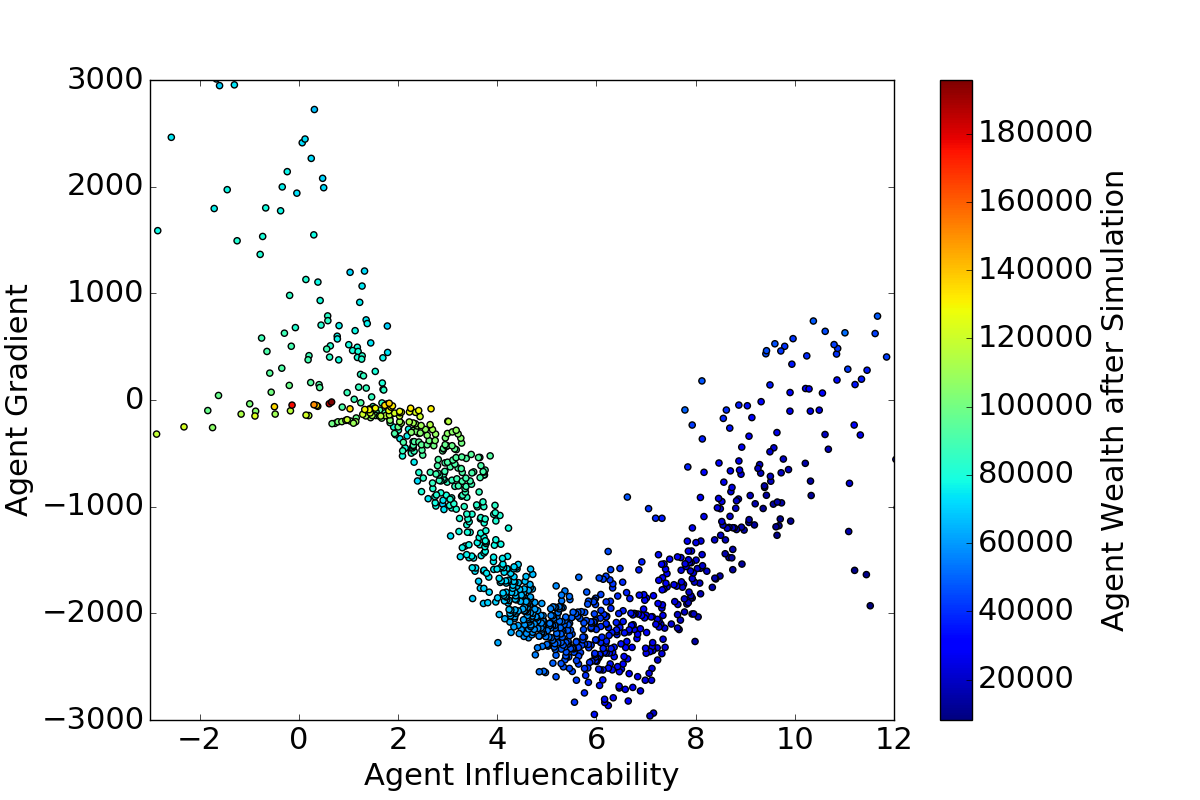
\includegraphics[width=0.45\textwidth]{figures/heuristic_gradient_example_2.png}
  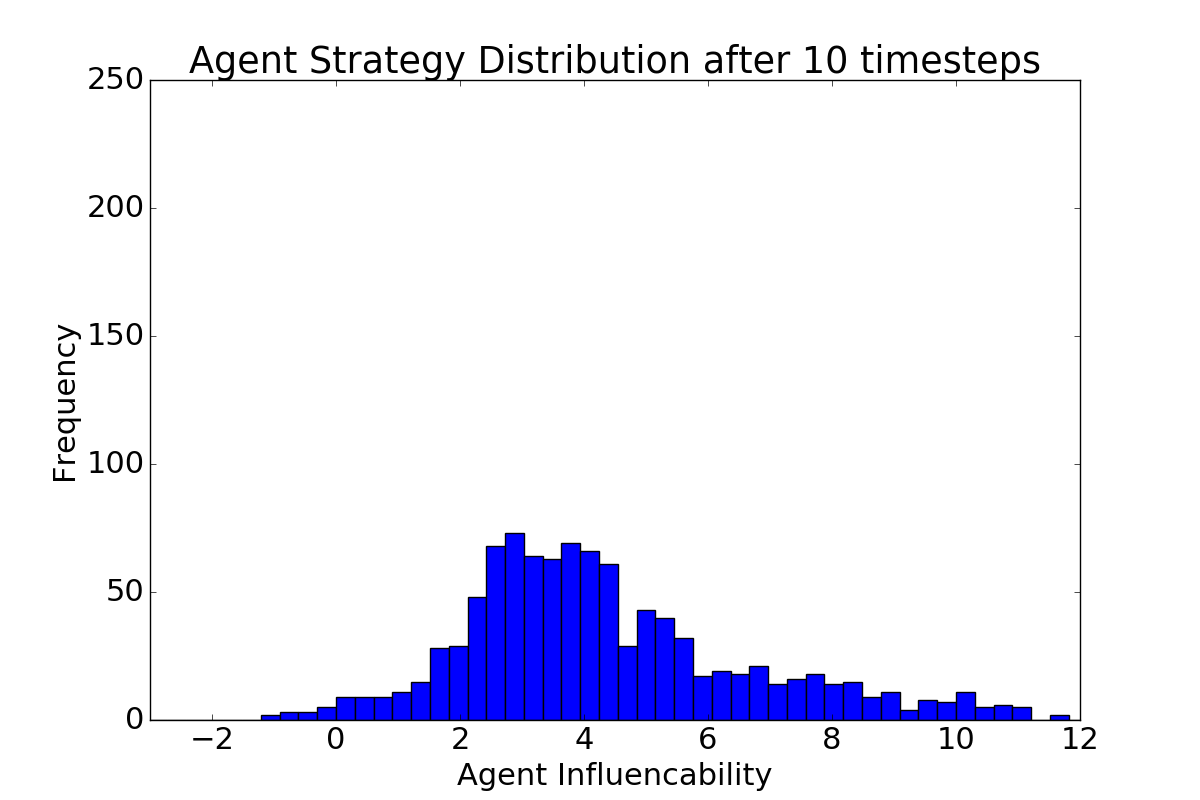
\includegraphics[width=0.45\textwidth]{figures/heuristic_gradient_example_3.png}
  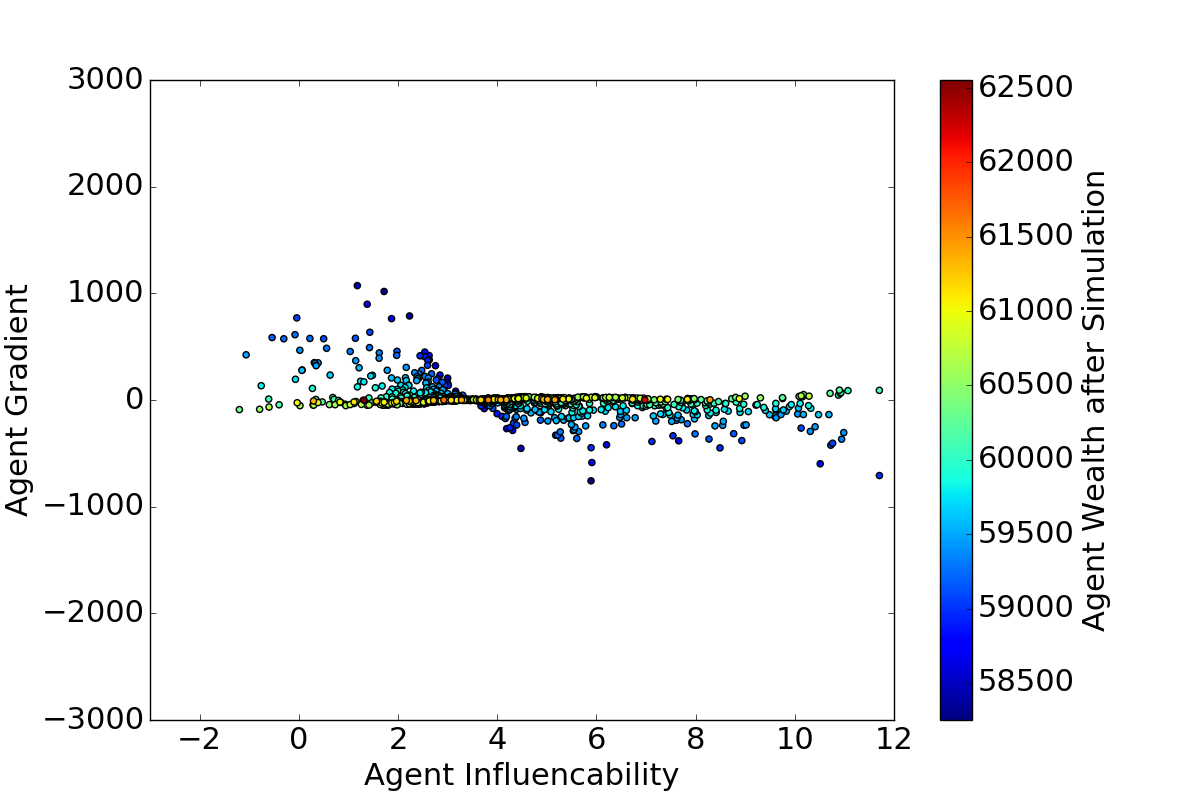
\includegraphics[width=0.45\textwidth]{figures/heuristic_gradient_example_4.png}
  \caption[Examples Heuristic Gradient]{Two examples where the simulation was run for a given 1D agent strategy distribution (left) and the corresponding agent gradients were computed (right). In the first example one can clearly see most agents having a negative gradient as the most successfull agents were the ones with smallest influencability. The second example shows a more symmetric gradient distribution.}
  \label{fig:heuristicgradient}
\end{figure}

\section{Implementation}
DANIEL

\section{Simulation Results and Discussion}
for simulation: DANIEL
* price formation: buy+sell curves
* price evolution: show graph
* justification of model: return evolution, show fat tail distribution

Running MLS turns out to be computationally very expensive. The amount of time steps needed to reach an equilibrium distribution was about the same for the few examples we ran (as can be seen in figure \ref{fig:heuristicvsmls}), but the computation time was much longer. Thus in the scope of this project it was decided to use the Heuristic Gradient method, as simulation times using Heuristic Gradient were very long already (around 10 hours for 300 learning steps). \\
\begin{figure}
  \centering
  \quad
  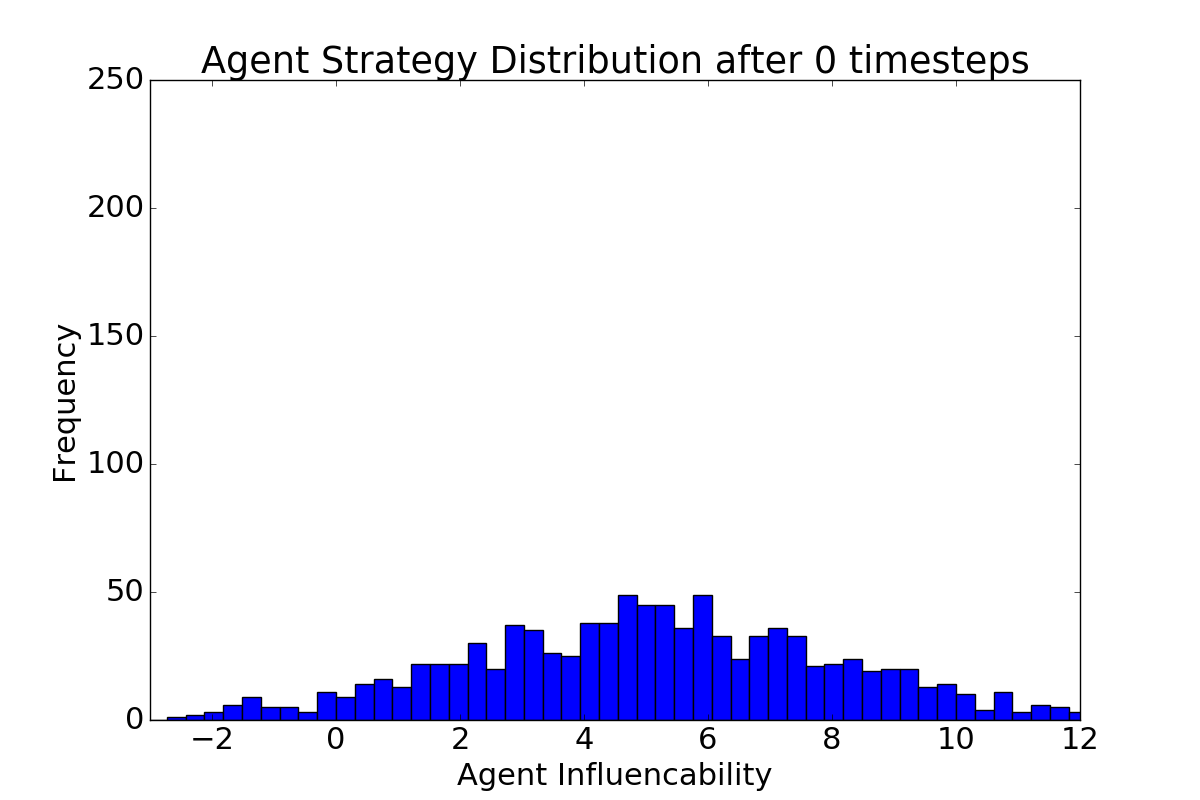
\includegraphics[width=0.45\textwidth]{figures/heuristic_vs_mls_1.png}
  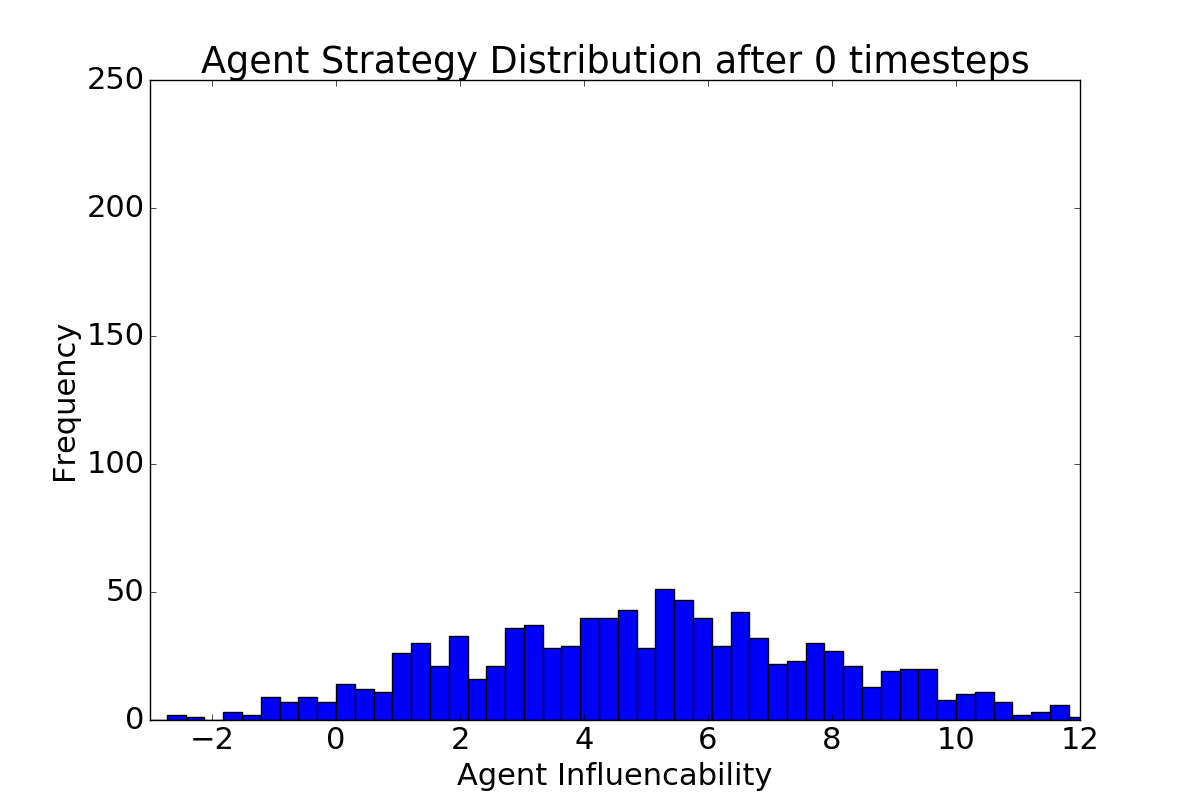
\includegraphics[width=0.45\textwidth]{figures/heuristic_vs_mls_4.png}
  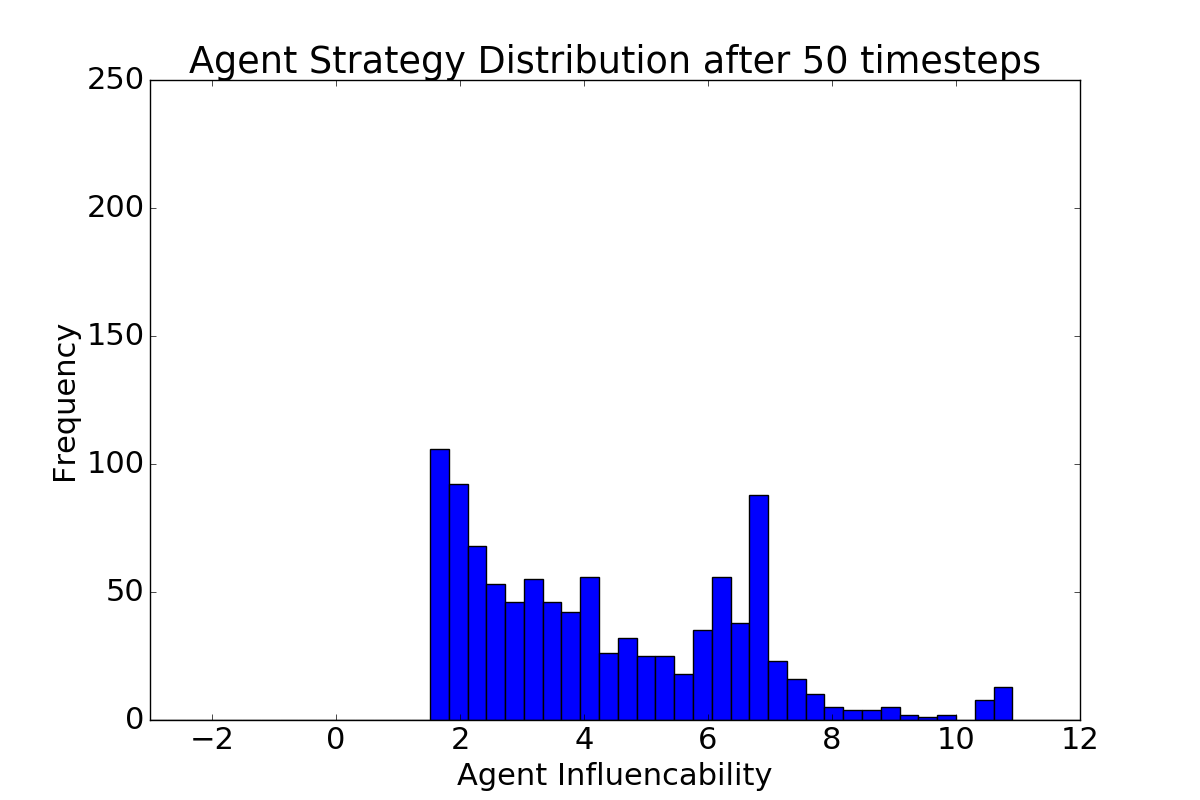
\includegraphics[width=0.45\textwidth]{figures/heuristic_vs_mls_2.png}
  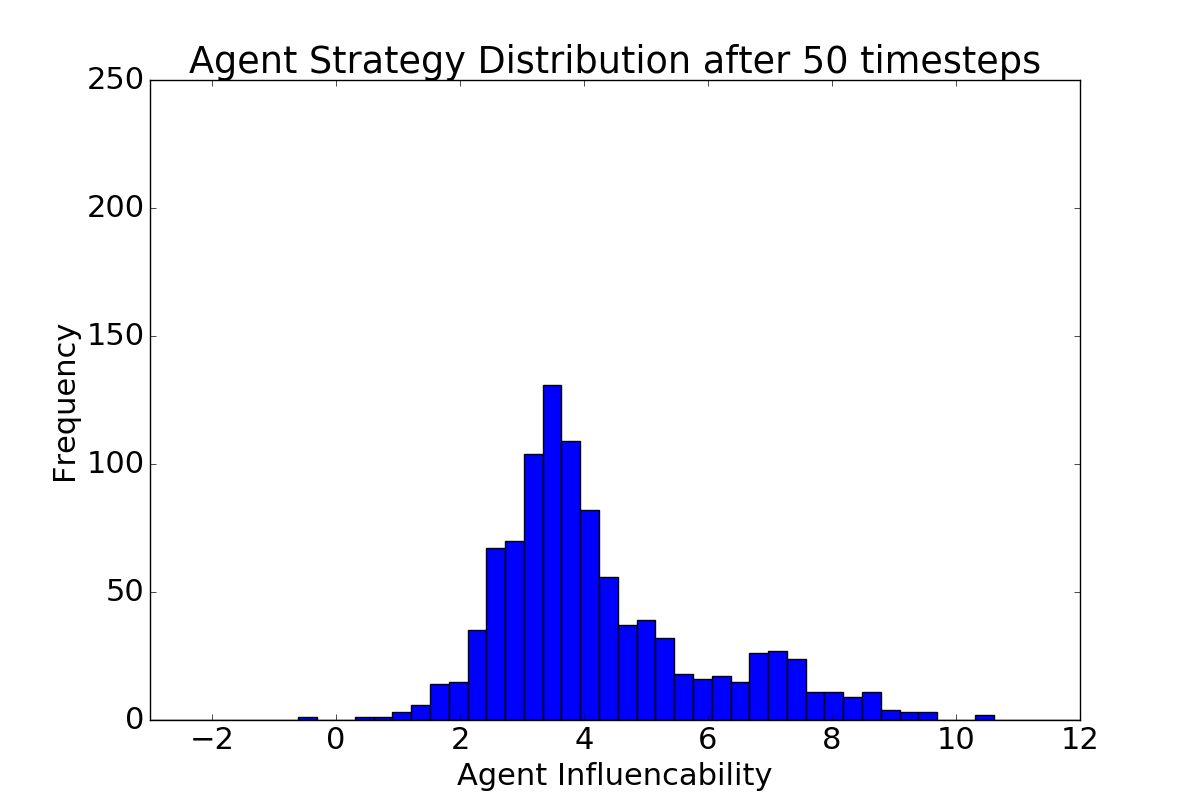
\includegraphics[width=0.45\textwidth]{figures/heuristic_vs_mls_5.png}
  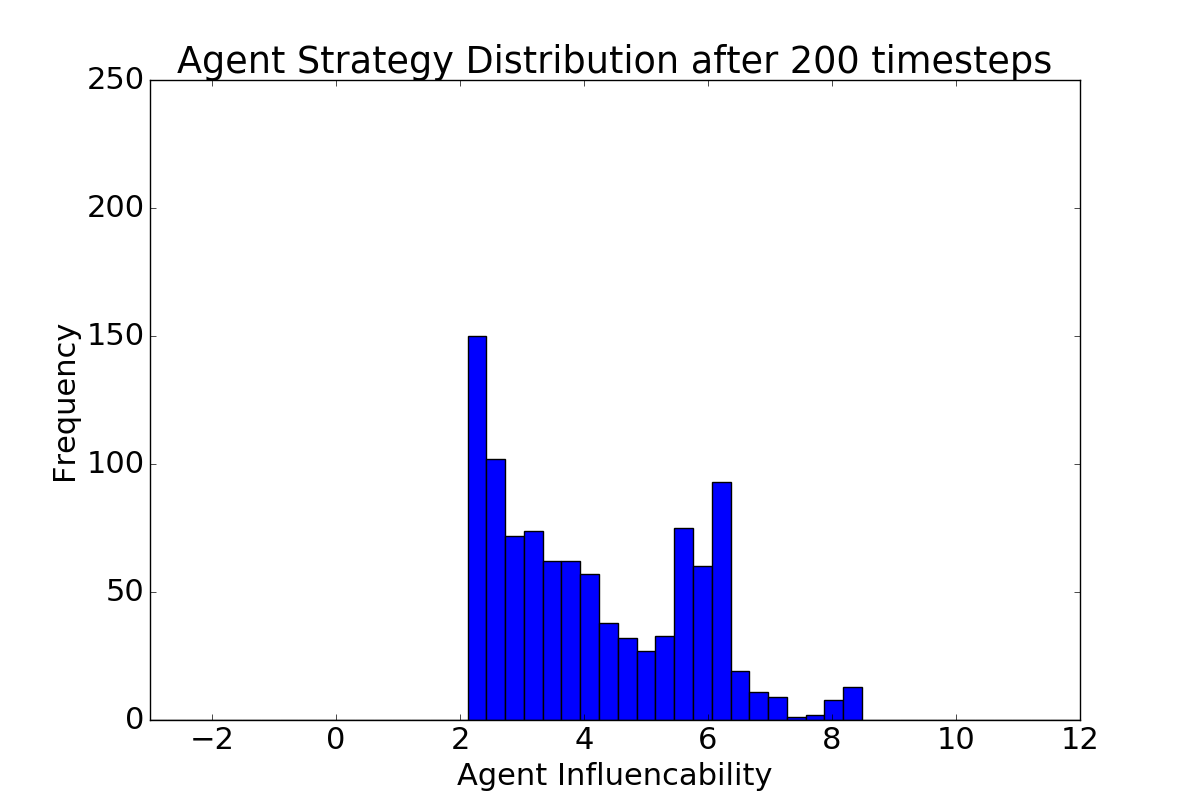
\includegraphics[width=0.45\textwidth]{figures/heuristic_vs_mls_3.png}
  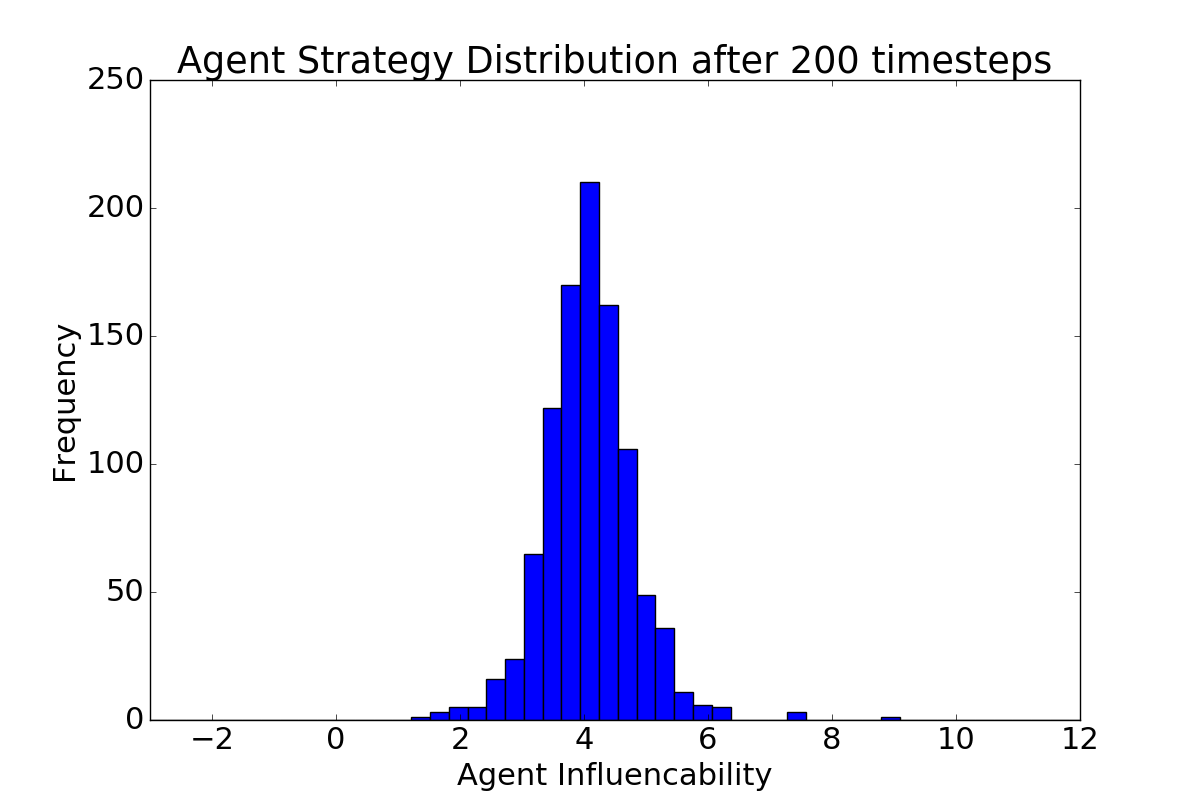
\includegraphics[width=0.45\textwidth]{figures/heuristic_vs_mls_6.png}
  \caption[Comparison MLS and Heuristic Gradient]{Simulation result of the MLS (left) and Heuristic Gradient (right) methods for the same inital agent distributions after 0, 50 and 200 timesteps. Both methods reached a stable distribution at around 150 timesteps.}
  \label{fig:heuristicvsmls}
\end{figure}
Additionally it was decided to reduce the agent parameter space to one dimension, as 2D (or even 3D simulation if the agent noisiness is not fixed) simulations need more learning steps and/or lower learning parameter. This can be seen in figure \ref{fig:2dsimulation} where a 2D simulation was run for 1000 learning steps. Even though the shrinking shape of the agent parameter distribution suggests that it would converge at some point, that point is still not reached after 1000 learning steps. \\
To reduce the parameter space to 1D we bind influencability and conservativeness with following equation: 
\begin{equation}
  \text{conservativeness} = \frac{9 - \text{influencability}}{400}
\end{equation}
\begin{figure}
  \centering
  \quad
  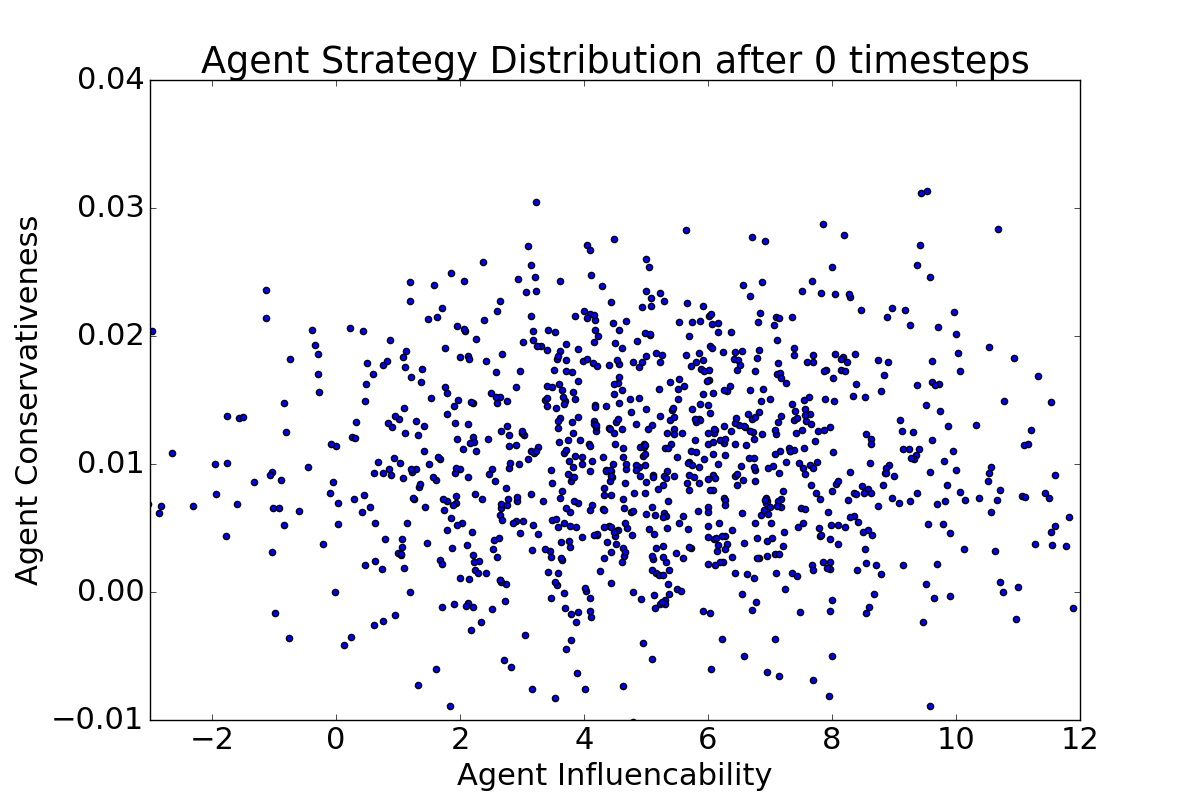
\includegraphics[width=0.31\textwidth]{figures/2dsim_1.png}
  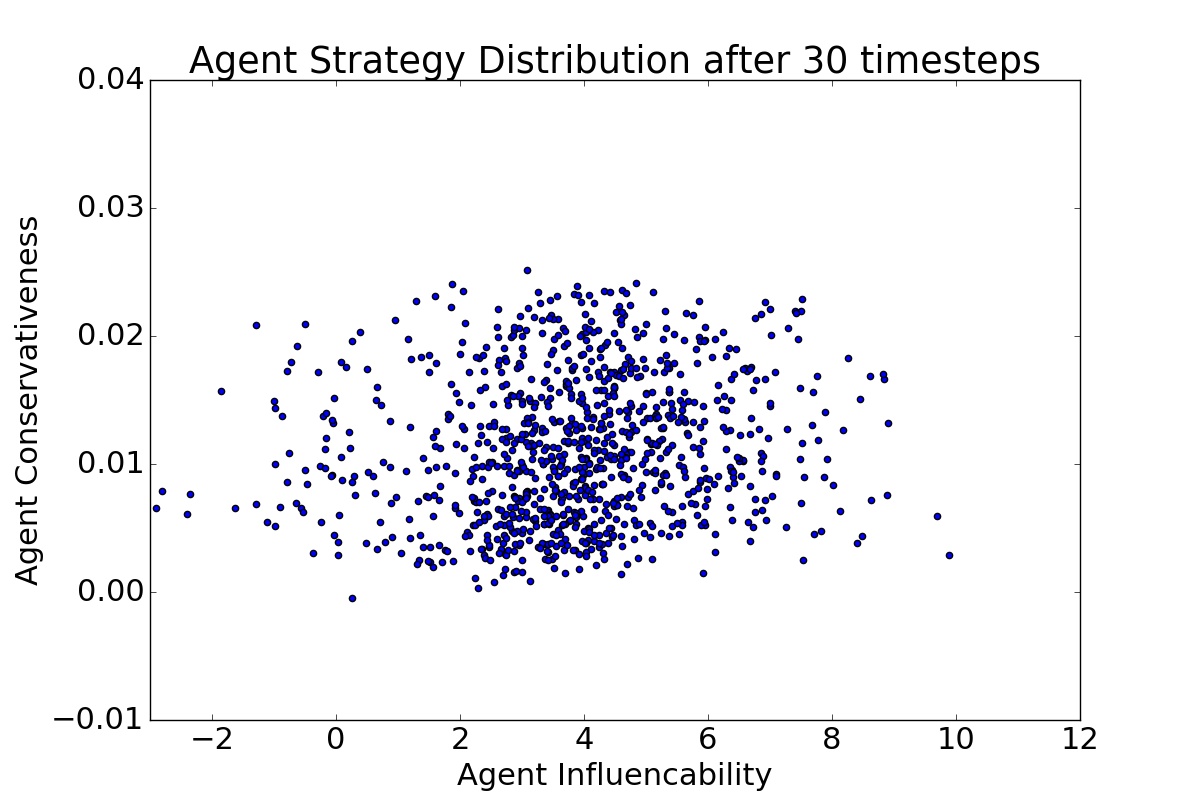
\includegraphics[width=0.31\textwidth]{figures/2dsim_2.png}
  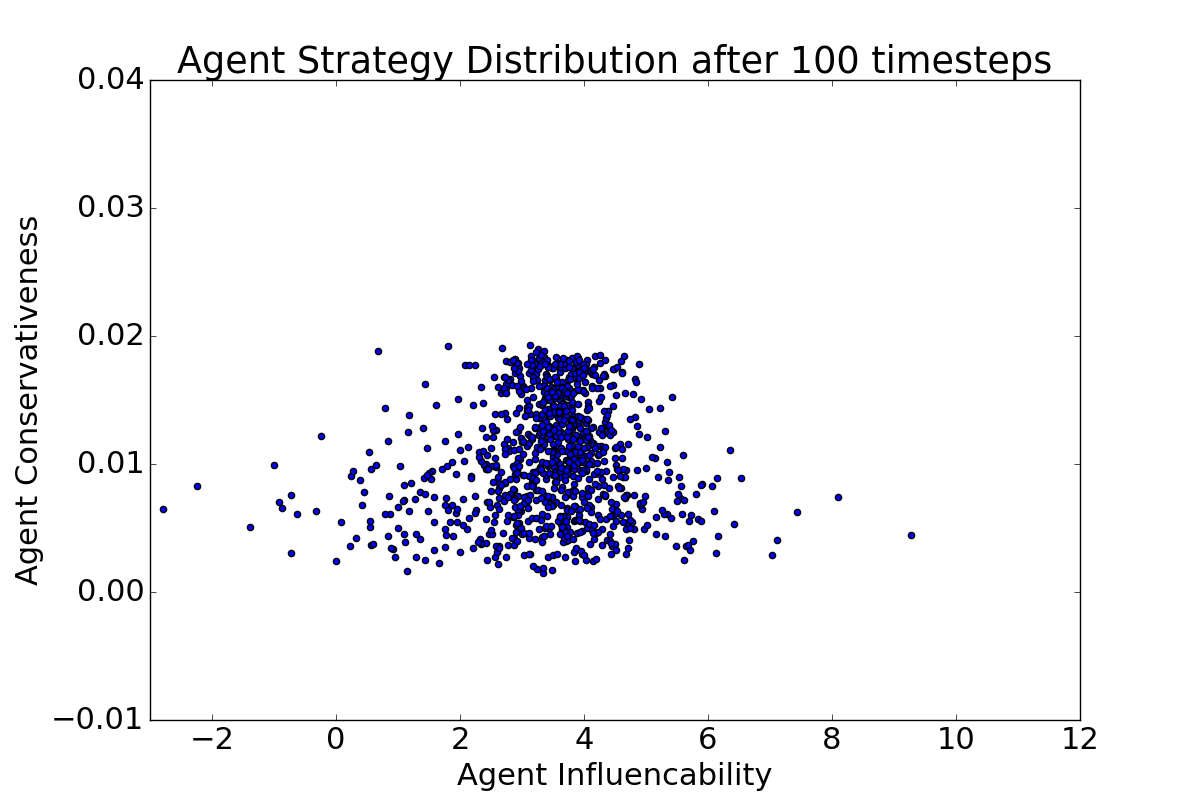
\includegraphics[width=0.31\textwidth]{figures/2dsim_3.png}
  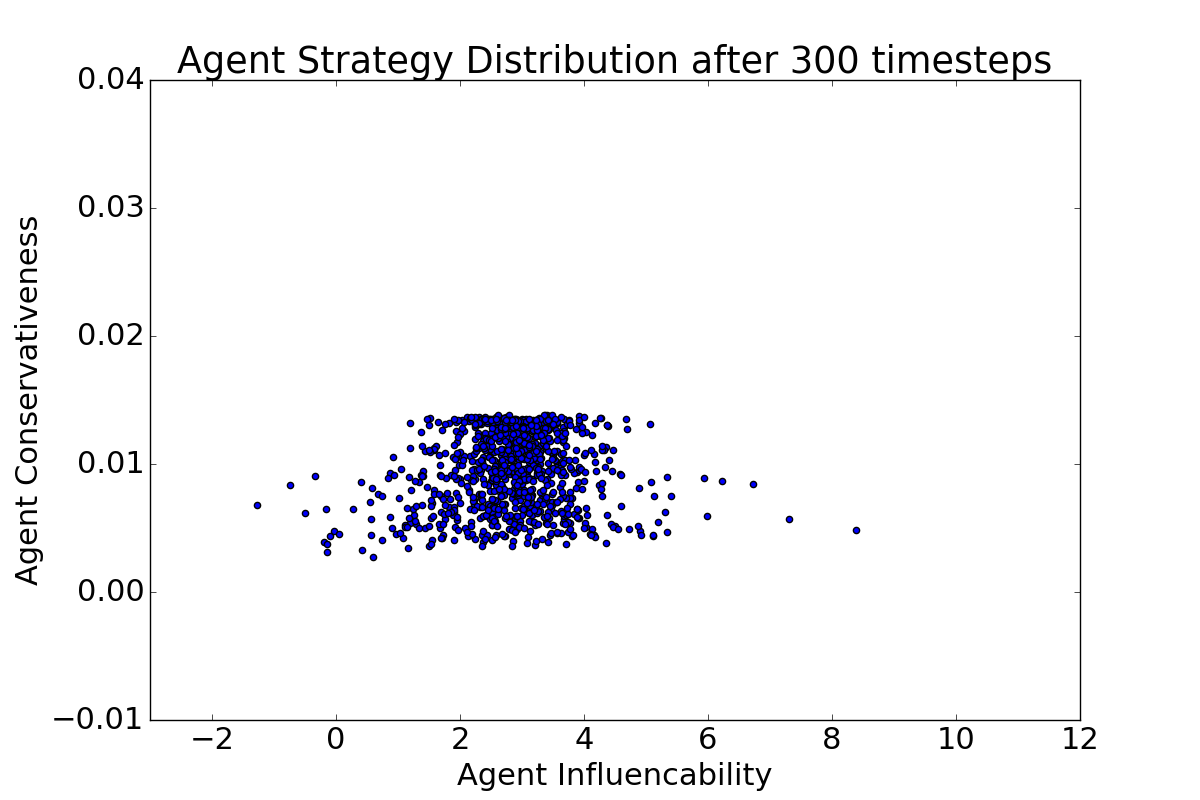
\includegraphics[width=0.31\textwidth]{figures/2dsim_4.png}
  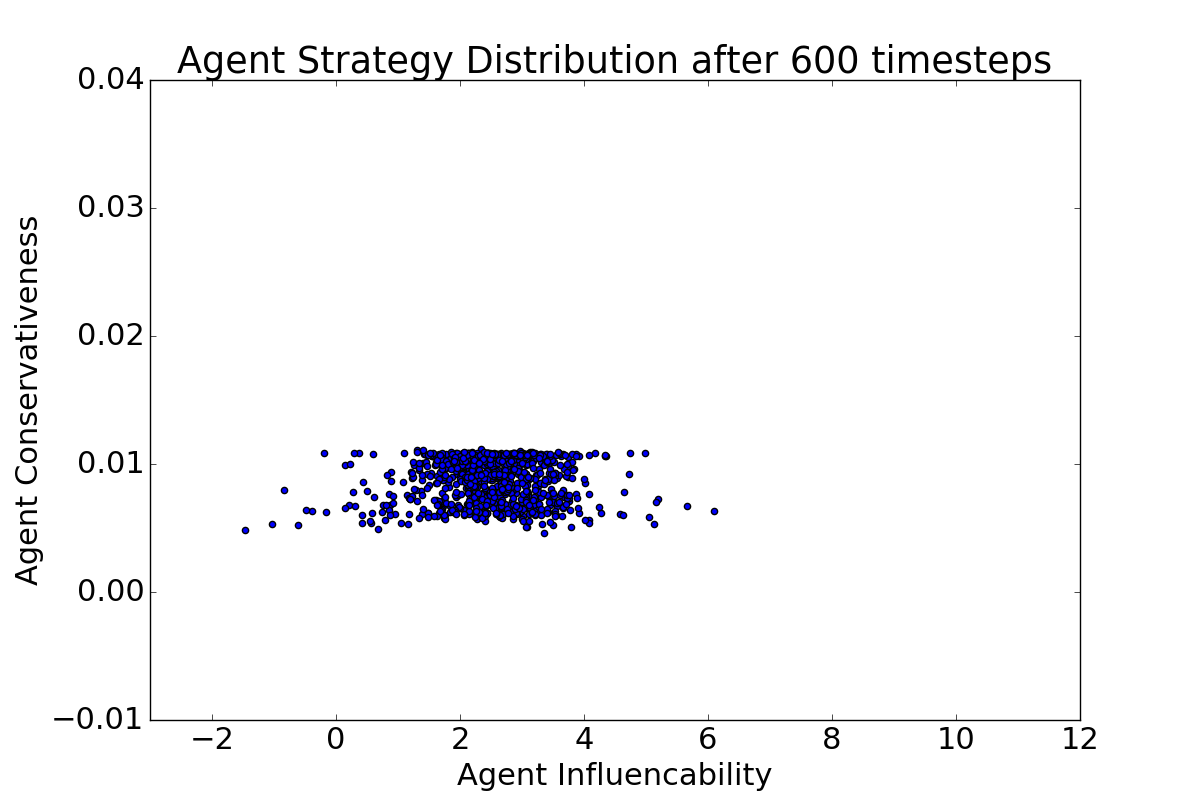
\includegraphics[width=0.31\textwidth]{figures/2dsim_5.png}
  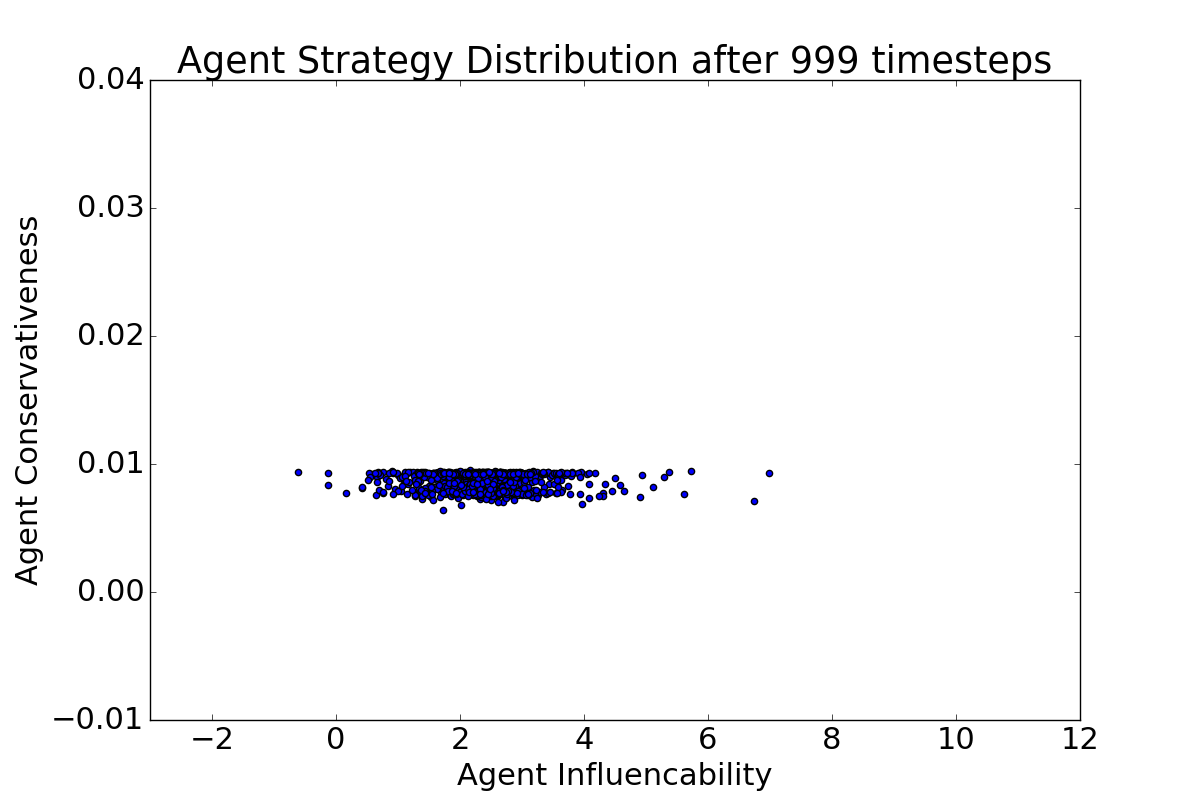
\includegraphics[width=0.31\textwidth]{figures/2dsim_6.png}
  \caption[2D simulation]{Evolution of agent parameter distribution for a Heuristic Gradient optimization in a 2D parameter space (conservativeness and influencability). Even after 1000 learning steps the distribution has not converged, as the shape is still changing.}
  \label{fig:2dsimulation}
\end{figure}

\hfill \\
All folowing simulations are done with the heuristic gradient method in the reduced 1D agent parameter space. One example of such a learning process is visualized in figure \ref{fig:convergenceexample}. In this case the initial agent distribution was chosen to be normally distributed with mean 5 and standard deviation 3. As one can see the strategy distribution converges to a stable gaussian-like shape. This convergence behaviour is analyzed if firstly it is consistently reproducible and secondly if it depends on  the inital strategy distribution of the agents. \\
\begin{figure}
  \centering
  \quad
  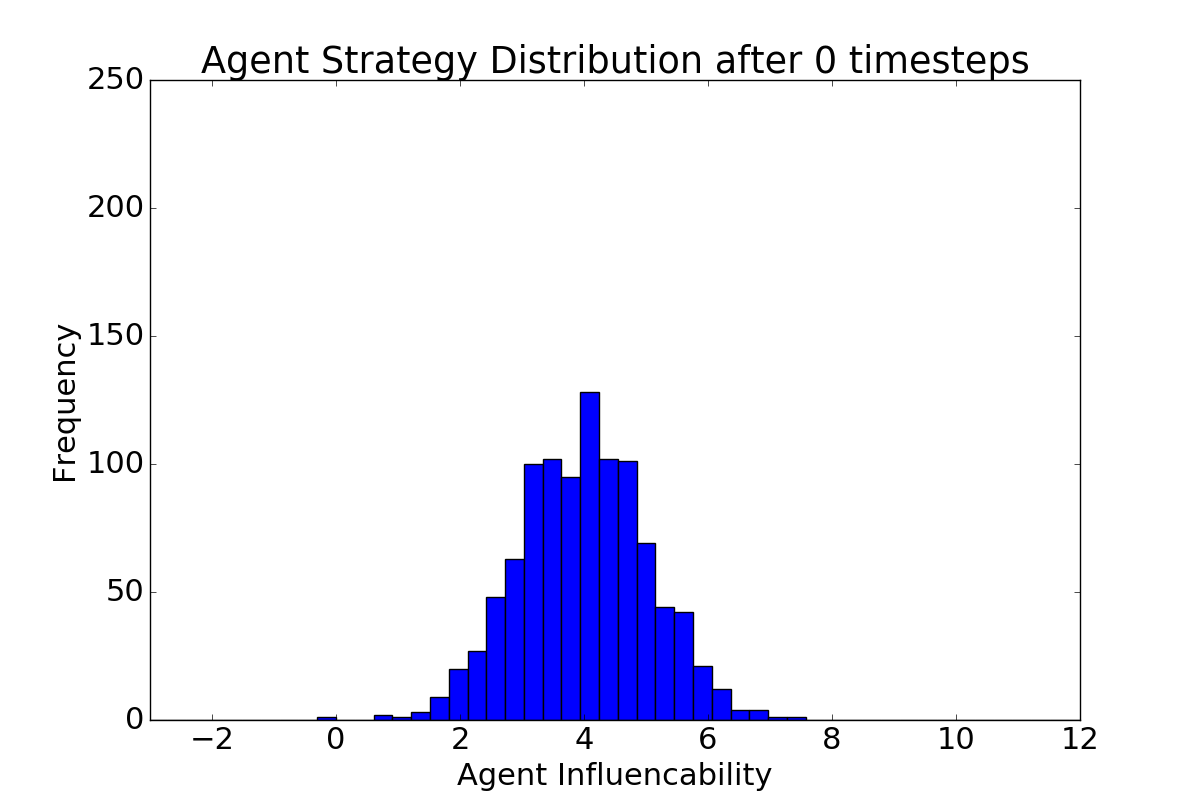
\includegraphics[width=0.45\textwidth]{figures/convergence_example_1.png}
  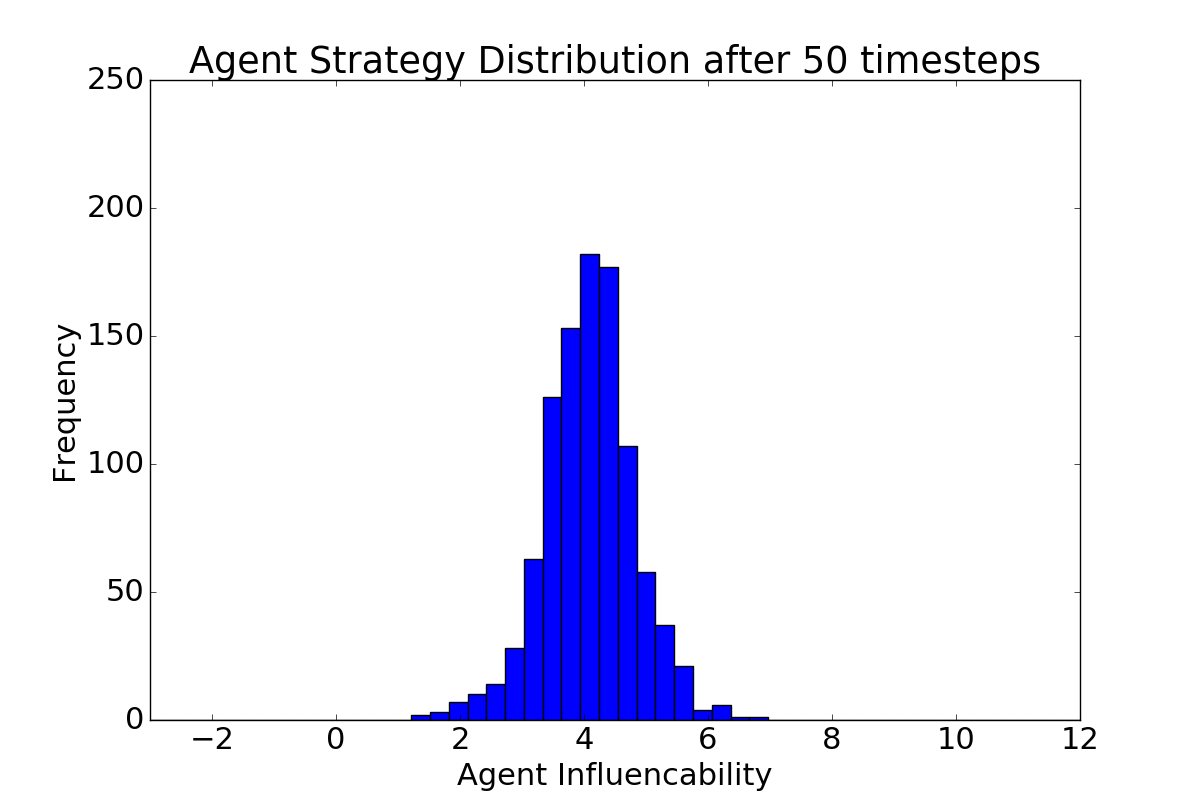
\includegraphics[width=0.45\textwidth]{figures/convergence_example_2.png}
  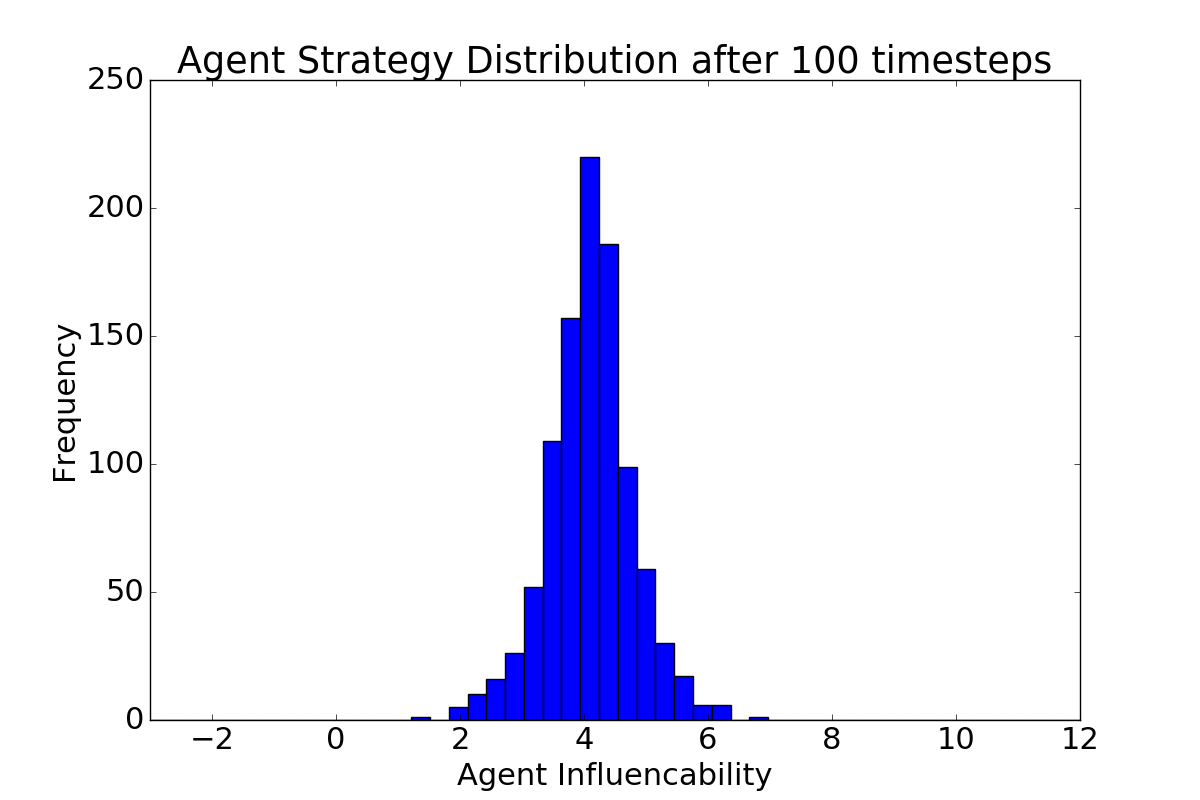
\includegraphics[width=0.45\textwidth]{figures/convergence_example_3.png}
  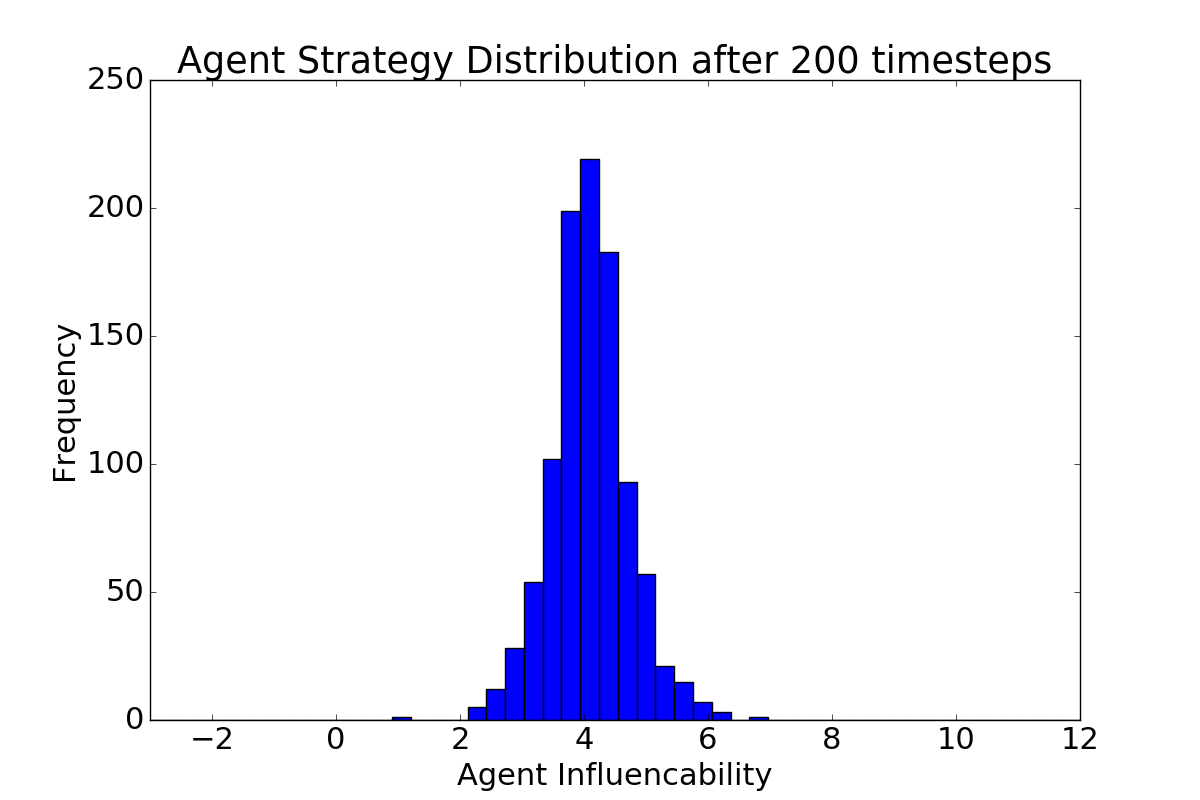
\includegraphics[width=0.45\textwidth]{figures/convergence_example_4.png}
  \caption[Convergence Example]{Results of a 1D Heuristic Gradient simulation with initial parameter distribution being normal with mean 5 and standard deviation 3. After around 100 timesteps the distribution converges to a gaussian-like shape and stays that way.}
  \label{fig:convergenceexample}
\end{figure}
The simulation is therefore ran 10 times with the same initial distribution of agent paramaters and the same gaussian-like curve was always observed in all the final distributions. All those distributions are fitted against a gaussian function yielding us ten different values for the mean $\mu_{conv}$ and the standard deviation $\sigma_{conv}$. Computing the standard deviation of those two sets yields the result:
\begin{center}
  $\mu_{conv} = 4.07\pm 0.03$ \\
  $\sigma_{conv} = 0.53\pm 0.02$
\end{center}
The deviations being so small indicate a high reproducability of the result. This gives us an idea of the uncertainty of the simulation result given an initial set of agents. This is very useful when one wants to investigate the dependence of the simulation result on the intial agent parameter distribution as we will below. \\
\hfill \\
35 Different simulations were run for different initial agent strategy distributions. The distributions were chosen to be normal with the mean and standard deviation being all possible permutations of $\mu=2,3,4,5,6,7,8$ and $\sigma=1,2,3,4,5$. Some of those initial distributions can be seen in figure \ref{fig:initialconditions}. They span the complete sensible space of agent parameters: Markets with high amount of agents with negative influencability start producing nonsensical behaviour, as most agents try to do the opposite of all other agents. Similarly markets with many agents with influencability larger than 15 were observed to crash quickly, as price immediatly fell down to zero or skyrocketed to unreasonable values. \\
\begin{figure}
  \centering
  \quad
  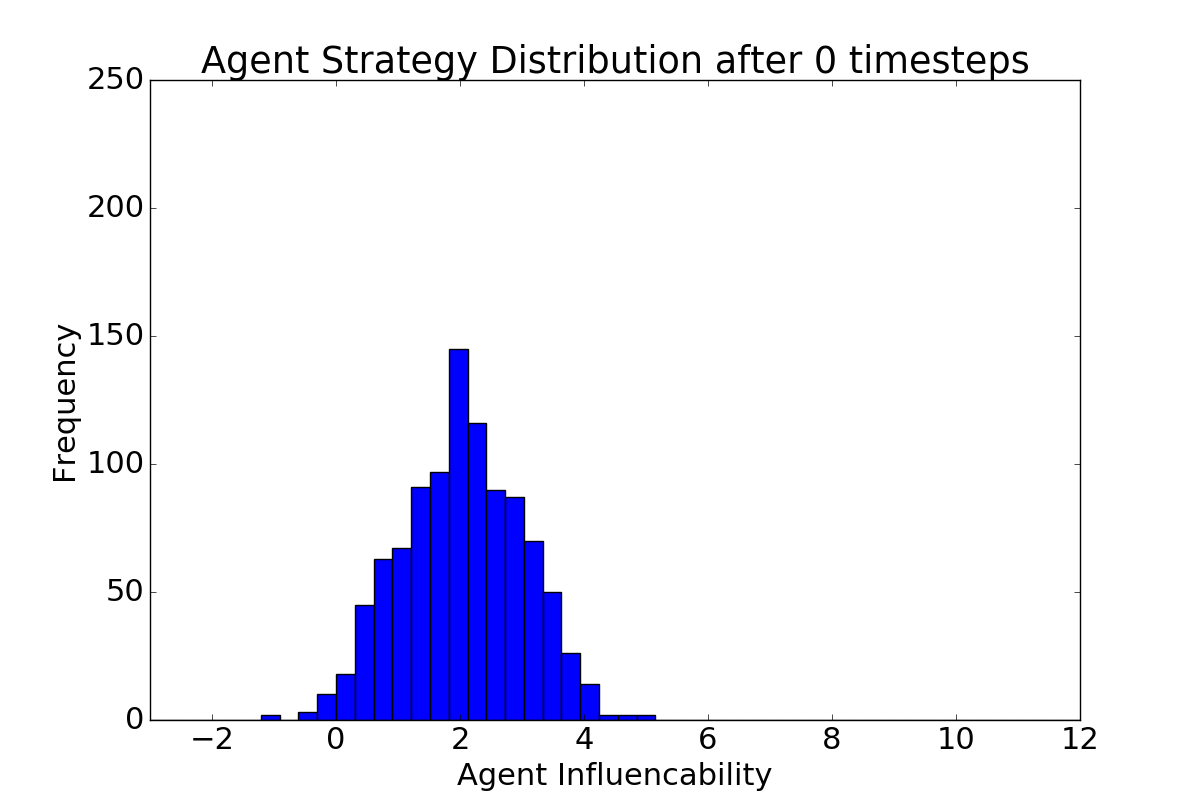
\includegraphics[width=0.3\textwidth]{figures/ic1.png}
  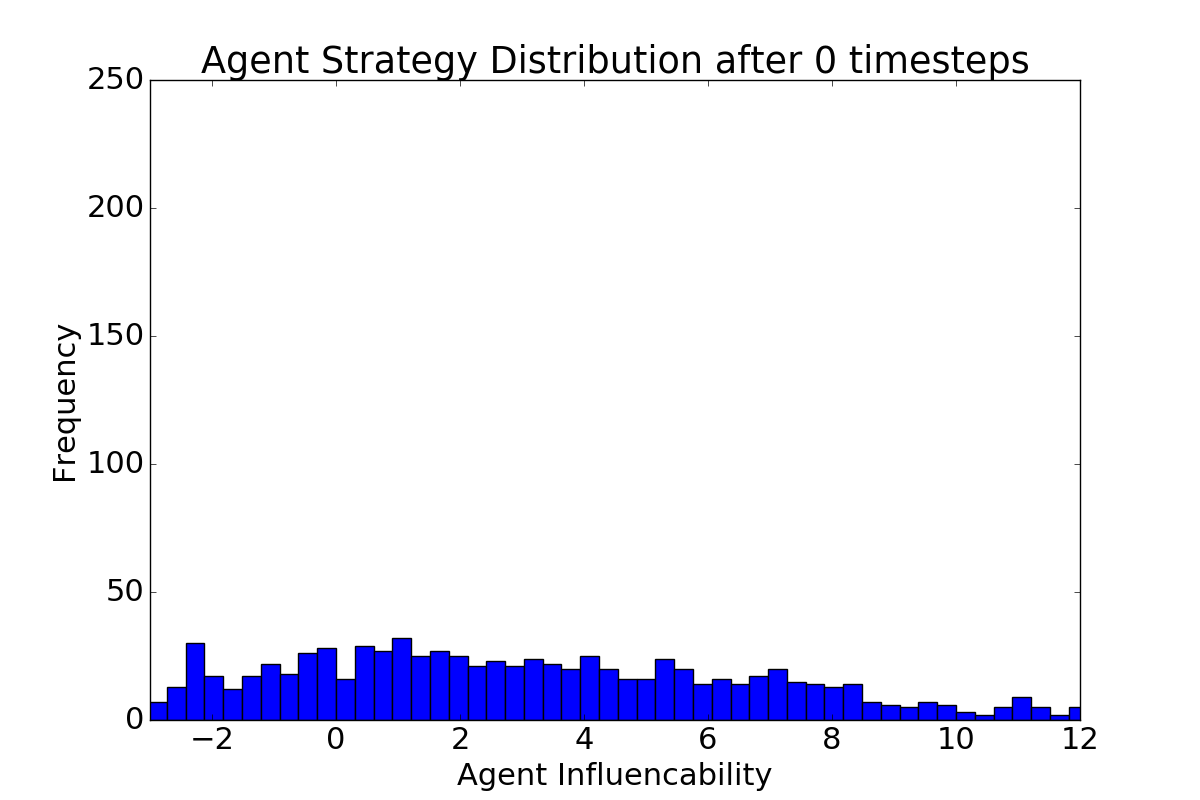
\includegraphics[width=0.3\textwidth]{figures/ic2.png}
  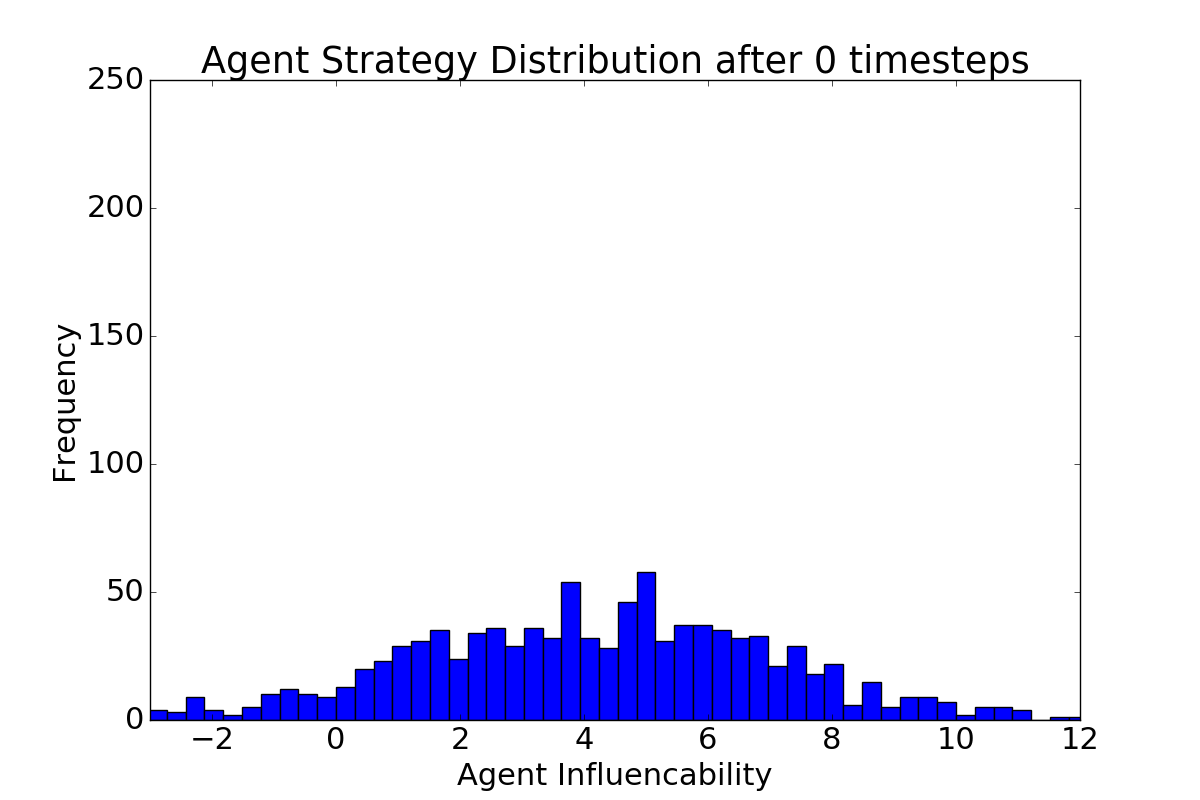
\includegraphics[width=0.3\textwidth]{figures/ic3.png}
  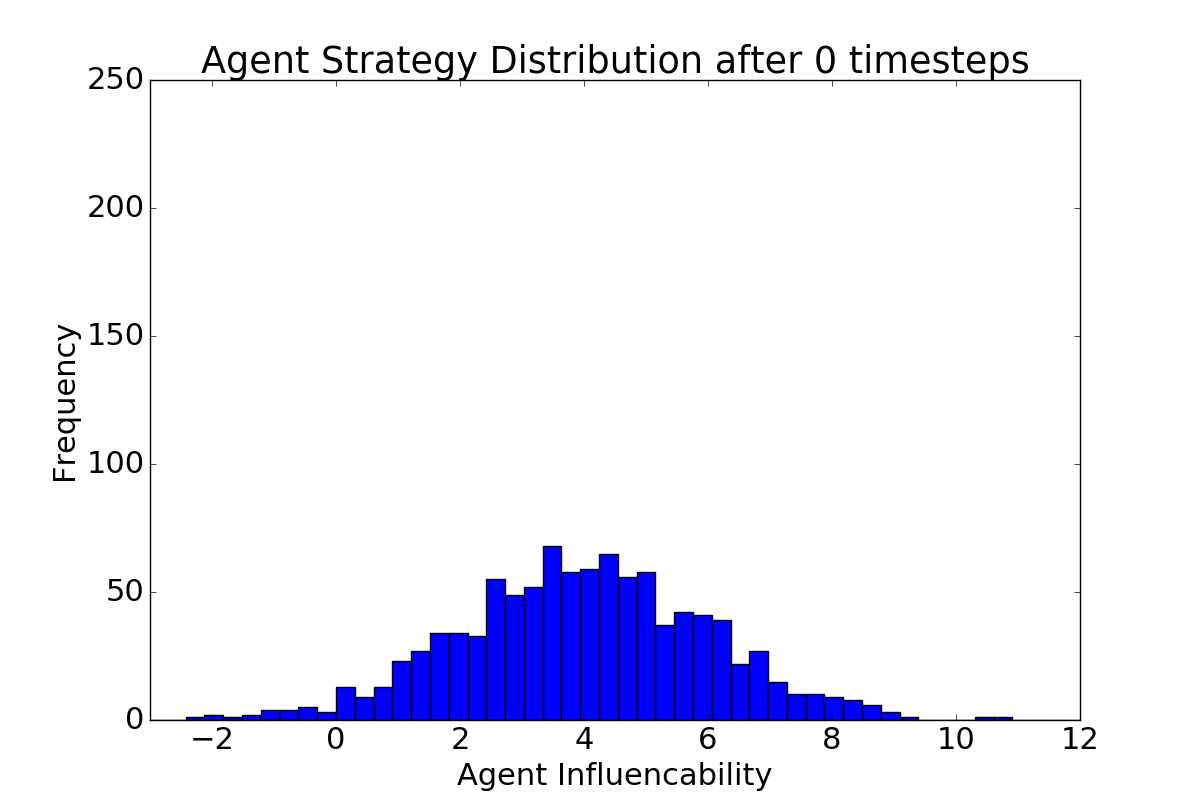
\includegraphics[width=0.3\textwidth]{figures/ic4.png}
  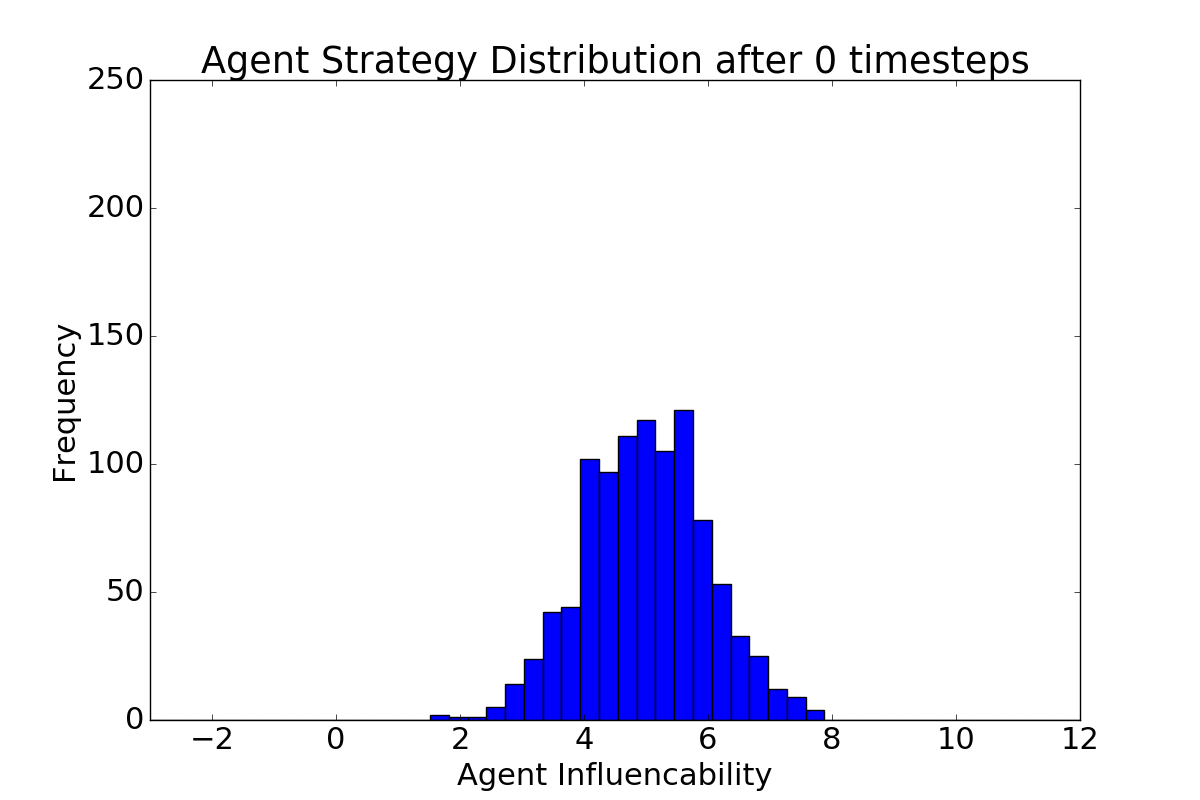
\includegraphics[width=0.3\textwidth]{figures/ic5.png}
  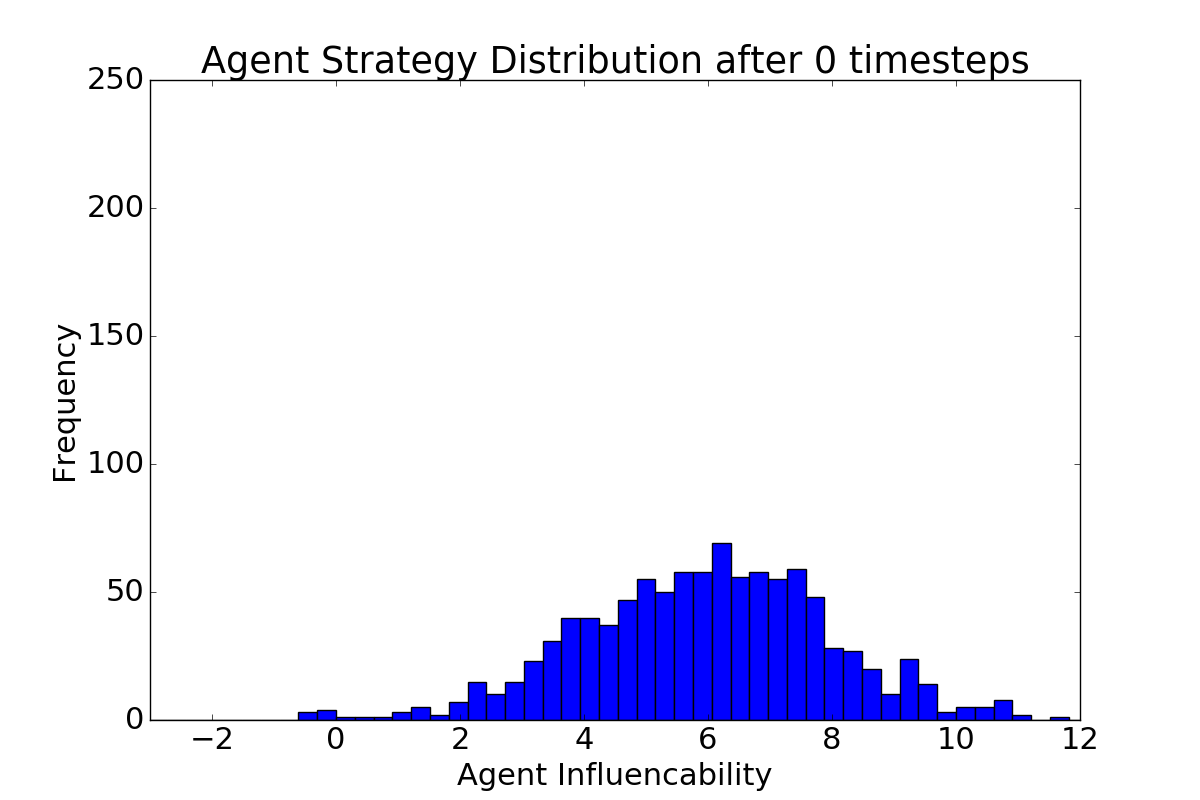
\includegraphics[width=0.3\textwidth]{figures/ic6.png}
  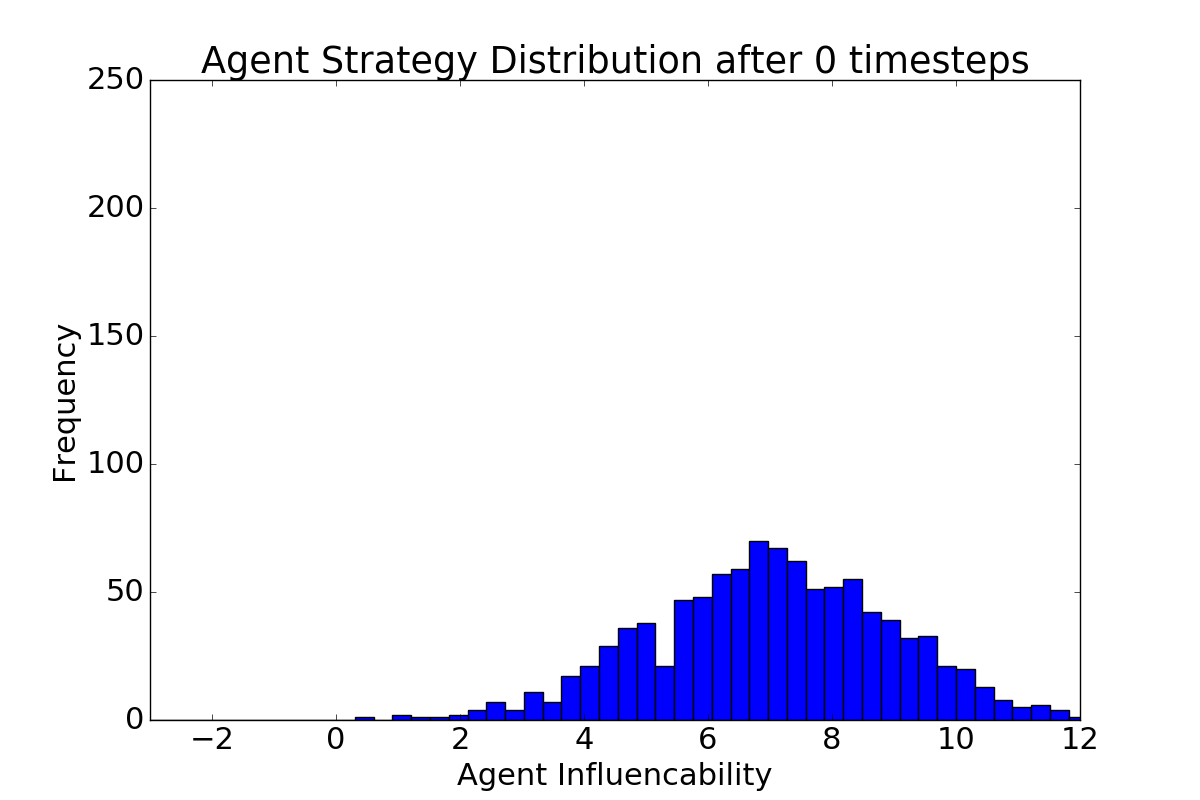
\includegraphics[width=0.3\textwidth]{figures/ic7.png}
  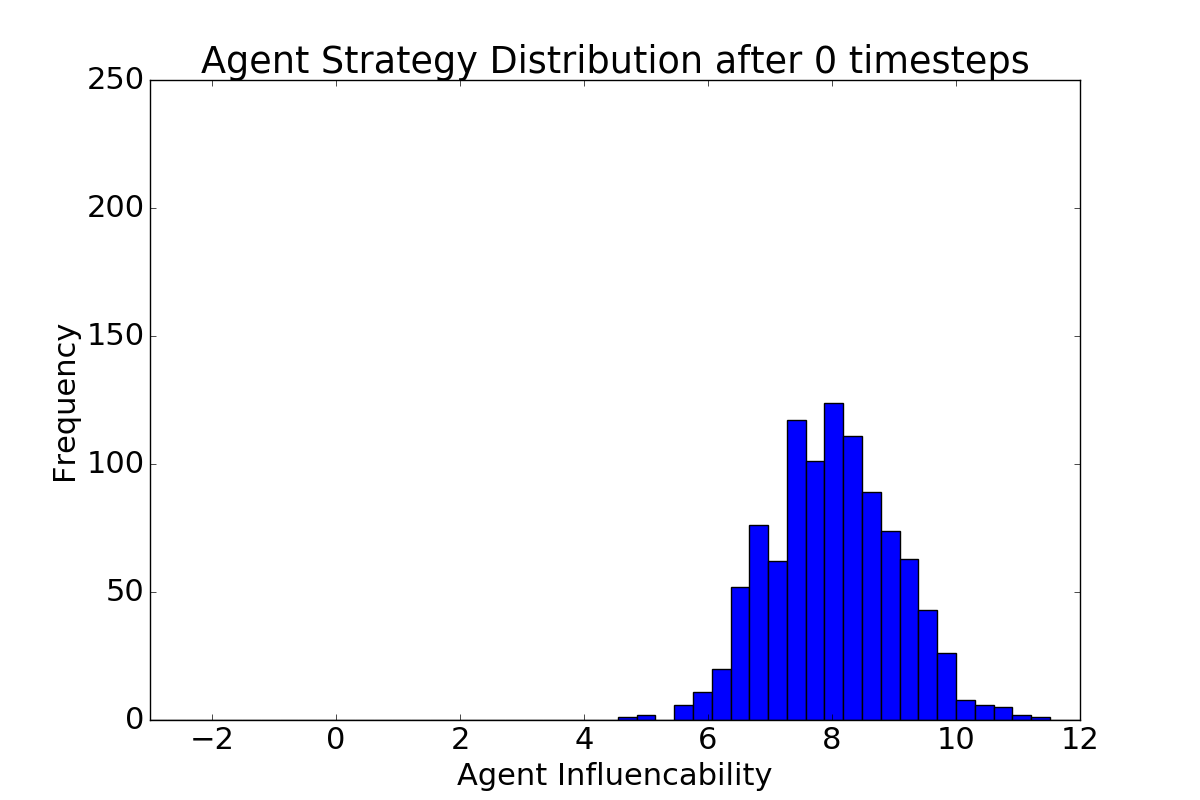
\includegraphics[width=0.3\textwidth]{figures/ic8.png}
  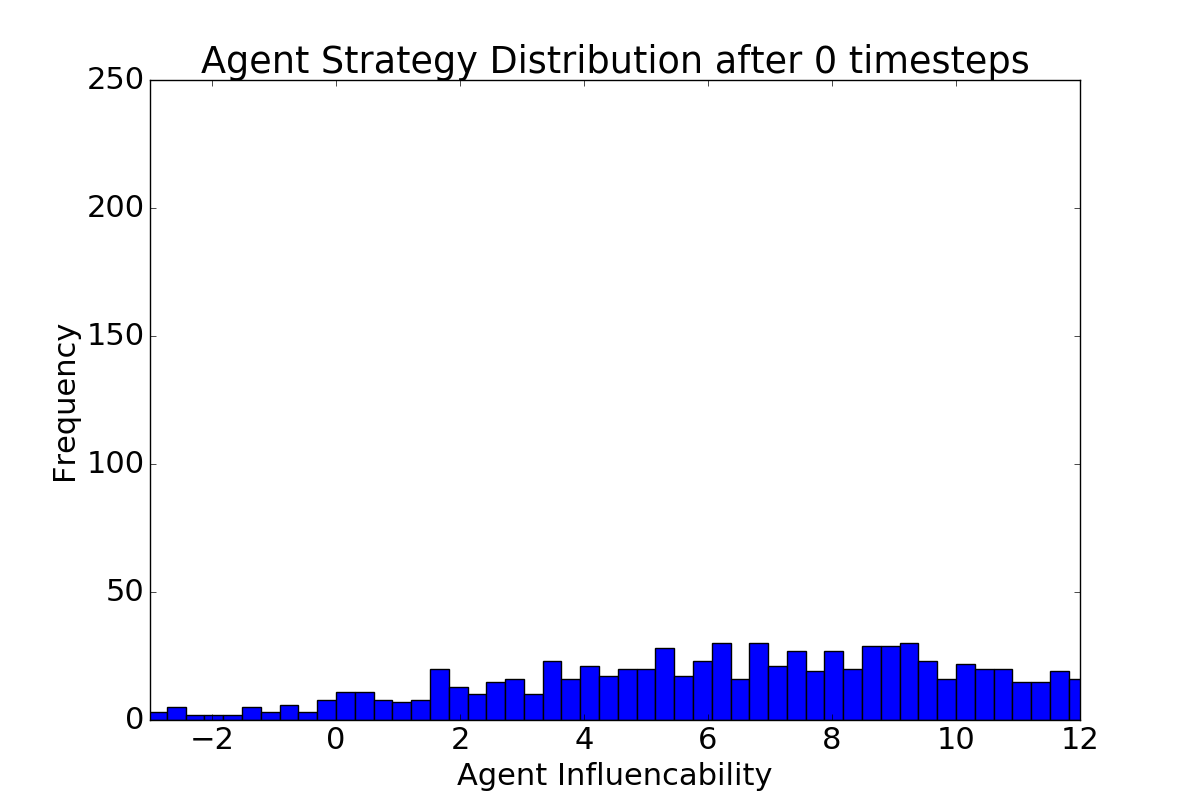
\includegraphics[width=0.3\textwidth]{figures/ic9.png}
  \caption[Different Initial Conditions]{9 of the 35 tested initial agent strategy distributions are plotted.}
  \label{fig:initialconditions}
\end{figure}
For all 35 different inital conditions the agent distribution converged to the same gaussian-like curve. Analogously as before those curves were fitted resulting in
\begin{center}
  $\mu_{conv} = 4.09\pm 0.07$
  $\sigma_{conv} = 0.52\pm 0.03$
\end{center}
These numbers are very similar to those observed in the reproducibility experiment, leading to the conclusions that our system always converges to the same strategy distribution.

\section{Summary and Outlook}
First we developed an agent-based model for financial market that is able to produce a wide variety of agent behaviour by introducing three agent parameters. We investigated an optimization process for a reduced agent parameter space that converged consistently to the same strategy distribution, independent of the initial distribution in a sensible range of agent parameters. This result is quite remarkable, as such a consitent outcome was not certain at all before running the simulations. However the precise shape of such a equilibrium distribution depends on the optimization process used. For example if the learning parameter would have been increased, one would expect the width of the equilibrium distribution to increase. Still there is an intrinsic property of our model independent on the learning algorithm that one can extract from our result: If the strategy distribution in a market adopts the gaussian-like shape that we discovered, then the ideal strategy for an agent is to appropriate the parameter value at the mean of the curve. Therefore we have in a certain way found an optimal strategy for the system. \\
\hfill \\
There are however still many areas that warrant further investigation of our model and our optimization process:
\begin{itemize}
  \item The restriction of the agent parameter space from 3D to 1D is completely arbitrary. Ideally one would want to run the optimization in all parameters, but this necessitates more computational power and time than available to us for our project.
  \item The optimization process should be investigated more thourougly. It is not a typical optimization process where one wants to find the extrema of a multivariate fitness function, because of two reasons: The output of our fitness function is stochastic and strongly depends on the other agent. The fitness function therefore changes slightly at each learning step as all the other agents change their parameters thus changing the market dynamics. Our optimization method naively ignores this fact. Therefore further research for more suitable mathematical methods is necessary.
  \item Our current result do not justify why our model and our optimization approach are sensible to model a real financial market. In contrary to other agent-based research works (e.g. \cite{raberto2001agent}) our invesetigation does not only aim to reproduce realistic emergent market behaviour, but also approximatively realistic agent behaviour. Justifying and analyzing a decision-making model is very difficult as there is only data what trade orders agents make, not why they make them. \\
  One way to still analyze our agents would be to make them compete in a market whose price history is taken from real market data, thus watching if our most successfull strategy would also be the most successfull in the real-world market. \\
  Another way to evaluate our model would be to fit real-world agent behaviour to our agent model by analyzing their trade orders and estimating their influencability, conservativeness and noisiness. One could then analyze how well those estimated agent parameter predict further trade orders of the real-world agent.
\end{itemize}


\section{References}
% load bibliography.bib
\bibliographystyle{abbrvnat}
\bibliography{bibliography}





\end{document}  



 
